\documentclass{ts_tech_doc}

\usepackage{algorithm}
\usepackage{algorithmicx}

%算法
%\begin{algorithm}[t]
%\caption{algorithm caption} %算法的名字
%\hspace*{0.02in} {\bf Input:} %算法的输入, \hspace*{0.02in}用来控制位置,同时利用 \\ 进行换行
%input parameters A, B, C\\
%\hspace*{0.02in} {\bf Output:} %算法的结果输出
%output result
%\begin{algorithmic}[1]
%\State some description % \State 后写一般语句
%\For{condition} % For 语句,需要和EndFor对应
%	\State ...
%	\If{condition} % If 语句,需要和EndIf对应
%		\State ...
%	\Else
%		\State ...
%	\EndIf
%\EndFor
%\While{condition} % While语句,需要和EndWhile对应
%	\State ...
%\EndWhile
%\State \Return result
%\end{algorithmic}
%\end{algorithm}

%!TEX root = ../ts_tech_doc_main.tex
% 文档信息

% 1. 文档中文标题
\titlecn{图迅科技5G物理层软件报价书}

% 2.文档英文标题
\titleen{Price quotation of 5G physical layer software of \\Toolsensing Co.,Ltd.}

% 3.文档日期
\thesisdate{year=2020,month=5}

\newif \ifblindreview % 条件语句,是否是盲审版本
% \blindreviewtrue
\blindreviewfalse

% lipsum
\newcommand{\lipsum} {
    
    这是一段随机插入的文本,用来填充模板布局,感受模板视觉效果。
    这是一段随机插入的文本,用来填充模板布局,感受模板视觉效果。
    这是一段随机插入的文本,用来填充模板布局,感受模板视觉效果。
}

\begin{document}
%%%%%%%%%%%%%%%%%%%%%%%%%%%%%%%%%%%%%%%%%%%%%%%%%%
% 封面
% -----------------------------------------------%
\makecoverpage

% %%%%%%%%%%%%%%%%%%%%%%%%%%%%%%%%%%%%%%%%%%%%%%%%%%
% % 前置部分的页眉页脚设置
% % -----------------------------------------------%
% \newpage
% % 正文和后置部分用阿拉伯数字编连续码,前置部分用罗马数字单独编连续码(封面除外)。
% % 设置封面页后的页码
% \pagenumbering{Roman} % 大写罗马字母
% \setcounter{page}{1} % 从1开始编号页码
% % 设置页眉和页脚 
% \pagestyle{fancy}
% % 正文以前部分无需页眉
% \fancyhf{} % 清空原有格式
% \renewcommand{\headrulewidth}{0pt}
% % 封面页无需页码,其他前置部分需要(按此理解扉页也是要页码的)。
% \fancyhf[CF]{\thepage} % 所有(奇数和偶数)中间页脚

% \ifblindreview	% 盲审不需要扉页和声明页
% \else
% %%%%%%%%%%%%%%%%%%%%%%%%%%%%%%%%%%%%%%%%%%%%%%%%%%
% % 扉页 
% % -----------------------------------------------%
% \maketitlepage
% \clearpage

% %%%%%%%%%%%%%%%%%%%%%%%%%%%%%%%%%%%%%%%%%%%%%%%%%%
% % 声明页
% % -----------------------------------------------%
% \announcement
% \clearpage
% \fi
% %%%%%%%%%%%%%%%%%%%%%%%%%%%%%%%%%%%%%%%%%%%%%%%%%%
% % 中文摘要
% % -----------------------------------------------%
% \section*{~}
% \addcontentsline{toc}{section}{摘要}
% \include{content/abstractcn}
% \clearpage

% %%%%%%%%%%%%%%%%%%%%%%%%%%%%%%%%%%%%%%%%%%%%%%%%%%
% % 英文摘要
% % -----------------------------------------------%
% \section*{~}
% \addcontentsline{toc}{section}{Abstract}
% \include{content/abstracten}
% \clearpage

%%%%%%%%%%%%%%%%%%%%%%%%%%%%%%%%%%%%%%%%%%%%%%%%%%
% 正文页眉页脚
% -----------------------------------------------%
\setcounter{page}{1} % 重置目录页码为小写罗马字体
\pagenumbering{roman} % 设置页码为小写罗马字体
% 设置页眉和页脚 %
\pagestyle{fancy}
\fancyhf[CF]{\thepage} % 所有(奇数和偶数)中间页脚

% 目录
% -------------------------------------------%
\section*{~}
\addcontentsline{toc}{section}{目录}   % 增加到目录中
{
    \renewcommand{\contentsname}{\hfill \heiti \zihao{3} 目\quad 录\hfill}
    \renewcommand*{\baselinestretch}{1.2}   % 行间距
    \tableofcontents
}
\newpage
% 去掉页眉章节序号后面的“.”
%\renewcommand{\sectionmark}[1]{\markright{\thesection~ #1}} 
\renewcommand{\sectionmark}[1]{\markboth{第\,\thesection\,章~~ #1}{}}% 显示章节号

\renewcommand{\headrulewidth}{1pt}
\fancyhf[ROH,REH]{\songti \zihao{5} \leftmark} % 设置所有(奇数和偶数)右侧页眉
\fancyhf[LEH,LOH]{\songti \zihao{5} 成都图迅科技有限公司} % 设置所有(奇数和偶数)左侧页眉
\fancyhf[CEF,COF]{\thepage} % 设置所有(奇数和偶数)中间页脚

% 正文内容 
% --------------------------------------------%
\setcounter{page}{1} % 重置页码编号
\pagenumbering{arabic} % 设置页码编号为阿拉伯数字

% 可以使用include命令导入tex文件,从而避免过多修改本文件。

% 文档正文是主体,主体部分应从另页右页开始,每一章应另起页。一般由序号标题、文字叙述、图、表格和公式等五个部分构成。

% 重新设置正文行间距,因为前置部分设置时候行间距被改过
\renewcommand*{\baselinestretch}{1.0}   % 几倍行间距
\setlength{\baselineskip}{20pt}         % 基准行间距

% 正文
{
    % 表格字号应比正文小,一般五号/10.5pt,但是暂时没法再cls里设置(不然会影响到封面等tabular环境)
    % 所以目前只好在主文件里局部\AtBeginEnvironment
    \AtBeginEnvironment{tabular}{\zihao{5}}
    %!TEX root = ../ts_docs_main.tex
% 文档正文是主体,主体部分应从另页右页开始,每一章应另起页。一般由序号标题、文字叙述、图、表格和公式等五个部分构成。
\section{图迅科技5G物理层技术规范}
\subsection{硬件与软件平台要求}

\begin{table}[htb]
    \centering
    \caption{图迅科技5G物理层软件运行软硬件要求}
    \label{T.example}
    \begin{tabular}{llllll}
        \hline
          & 建议硬件平台   & Intel Xeon D-2177NT \\
        \hline
          & 建议操作系统 & Centos 7 \\
        \hline
          & C++编译器 & GCC 7.5.0 \\
        \hline{}
    \end{tabular}
\end{table}


\subsection{5G物理层系统架构}

\begin{figure}[H]
    \centering
    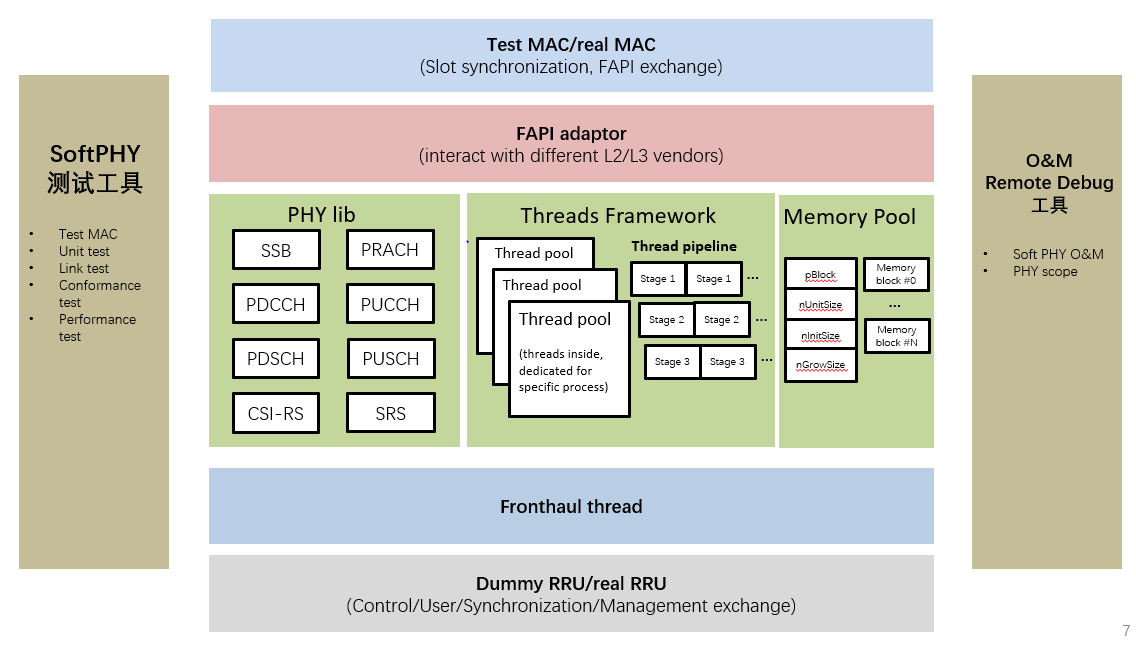
\includegraphics[width=0.8\textwidth]{图迅科技5G物理层软件架构.png}
    \caption{图迅科技5G物理层软件架构}
    \label{F.1_1}
\end{figure}

图迅科技的物理层软件系统结构如图\ref{F.1_1}所示。主要包括以下部分:

(1) Test/Real MAC: 用于模拟MAC层调度功能,调度物理层各信道。

(2) FAPI适配器(FAPI adaptor): 物理层与协议栈的FAPI接口适配器,将不同厂商的接口转换为标准的FAPI接口,以满足和不同协议栈厂商的对接。

(3) NR物理层软件(PHY Lib/ Threads Framework/ Memory Pool): 物理层软件的核心代码部分,主要包括物理层信道处理部分、线程池调度框架和内存池管理框架。其中物理层信道处理用于进行5G NR基带信号的调制和解调,线程池管理用于进行多线程的分配,管理和释放等操作,内存池管理主要用于所有物理层软件的内存统一管理。

\subsection{5G物理层软件功能}
\subsubsection{系统参数配置}

(1) 频段: 支持FR1。

(2) 子载波间隔: 支持30KHz子载波间隔配置。

(3) 带宽: 支持最大100MHz的带宽灵活配置。

(4) PHY-MAC接口: 基于Small Cell论坛的NR FAPI接口适配。

(5) 双工方式: 支持TDD和FDD,灵活支持各种TDD上下行时隙配比。

(6) 收发天线数: 支持1/2/4收发天线配置。

(7) 循环前缀类型: 支持Normal CP。

(8) BWP数量: 支持1个BWP(不包括初始接入BWP)。

(9) 激活UE数量: 支持256个激活用户。

(10) 每TTI调度用户数: 支持每TTI调度8个用户。

\subsubsection{物理信道功能}
图迅科技的物理层解决方案,支持的上下行物理信道功能描述如下:

(1) NR下行信道 

\begin{figure}[!htbp]
  \centering
  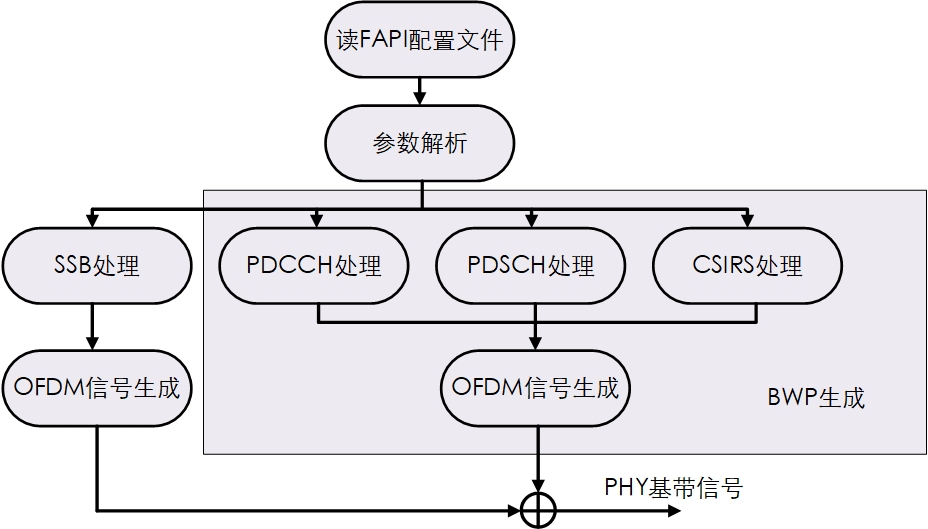
\includegraphics[width=0.8\textwidth]{nr_dl_process.jpg}
  \caption{图迅科技5G物理层软件下行处理流程图}
  \label{F.1_2}
\end{figure}

\par
\hangafter=0 %第一行缩进
\setlength{\hangindent}{2em}
NR下行信道支持基于3GPP协议版本f70的基带信号生成功能(图\ref{F.1_2}),其组成部分包括:
\par
\hangafter=0 %第一行缩进
\setlength{\hangindent}{2em}
物理广播信道(PBCH)
\par
\hangafter=0 %第一行缩进
\setlength{\hangindent}{2em}
主同步信号(PSS)
\par
\hangafter=0 %第一行缩进
\setlength{\hangindent}{2em}
辅同步信号(SSS)
\par
\hangafter=0 %第一行缩进
\setlength{\hangindent}{2em}
物理下行共享信道(PDSCH)
\par
\hangafter=0 %第一行缩进
\setlength{\hangindent}{2em}
物理下行共享信道相关的解调参考信号(PDSCH DMRS)
\par
\hangafter=0 %第一行缩进
\setlength{\hangindent}{2em}
物理下行控制信道(PDCCH)
\par
\hangafter=0 %第一行缩进
\setlength{\hangindent}{2em}
物理下行控制信道相关的解调参考信号(PDCCH DMRS)
\par
\hangafter=0 %第一行缩进
\setlength{\hangindent}{2em}
信道状态信息参考信号(CSIRS)\\

A. SSB功能

\begin{figure}[h]
  \centering
  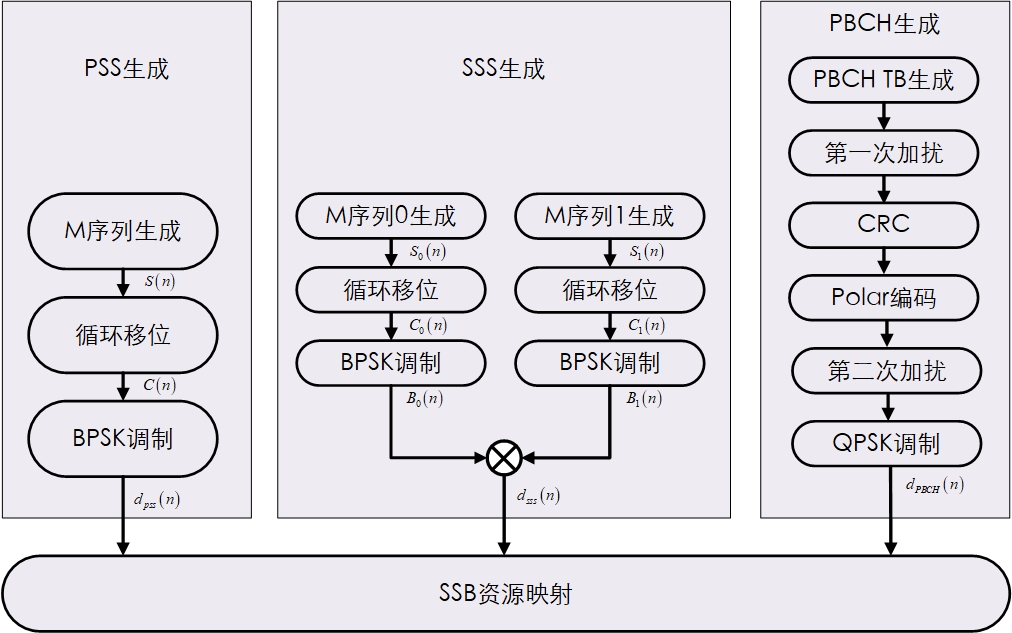
\includegraphics[width=0.85\textwidth]{nr_ssb_process.jpg}
  \caption{图迅科技5G物理层SSB处理流程图}
  \label{F.1_3}
\end{figure}

\par
\hangafter=0 %第一行缩进
\setlength{\hangindent}{2em}
如图\ref{F.1_3}所示,SSB信道的处理流程主要包括三大部分:PSS生成,SSS生成,PBCH生成,功能支持见表\ref{T.1_2}:

\begin{table}[h]
  \centering
  \caption{SSB主要功能列表}
  \label{T.1_2}
  \begin{tabular}{llllll}
      \hline
        & 功能   & 支持情况 \\
      \hline
        & L2参数解析 & 支持 \\
      \hline
        & SSB类型 & case A, case B, case C \\
      \hline
        & PSS 生成& 序列生成,资源映射 \\
      \hline
        & SSS 生成 & 序列生成,资源映射 \\
      \hline
        & PBCH 生成 & \makecell[l]{payload生成,第一次加扰,添加CRC, 信道编码, \\ 速率匹配, 第二次加扰, QPSK调制, 资源映射} \\
      \hline{}
  \end{tabular}
\end{table}


B. PDCCH功能

\par
\hangafter=0 %第一行缩进
\setlength{\hangindent}{2em}
如图\ref{F.1_4}所示,PDCCH信道处理根据CORESET配置信息和DCI配置信息进行下行控制信号的生成,PDCCH DMRS和下行DCI一起发送,用于该DCI的解调。下行PDCCH功能见表\ref{T.1_3}。\\

\begin{figure}[h]
  \centering
  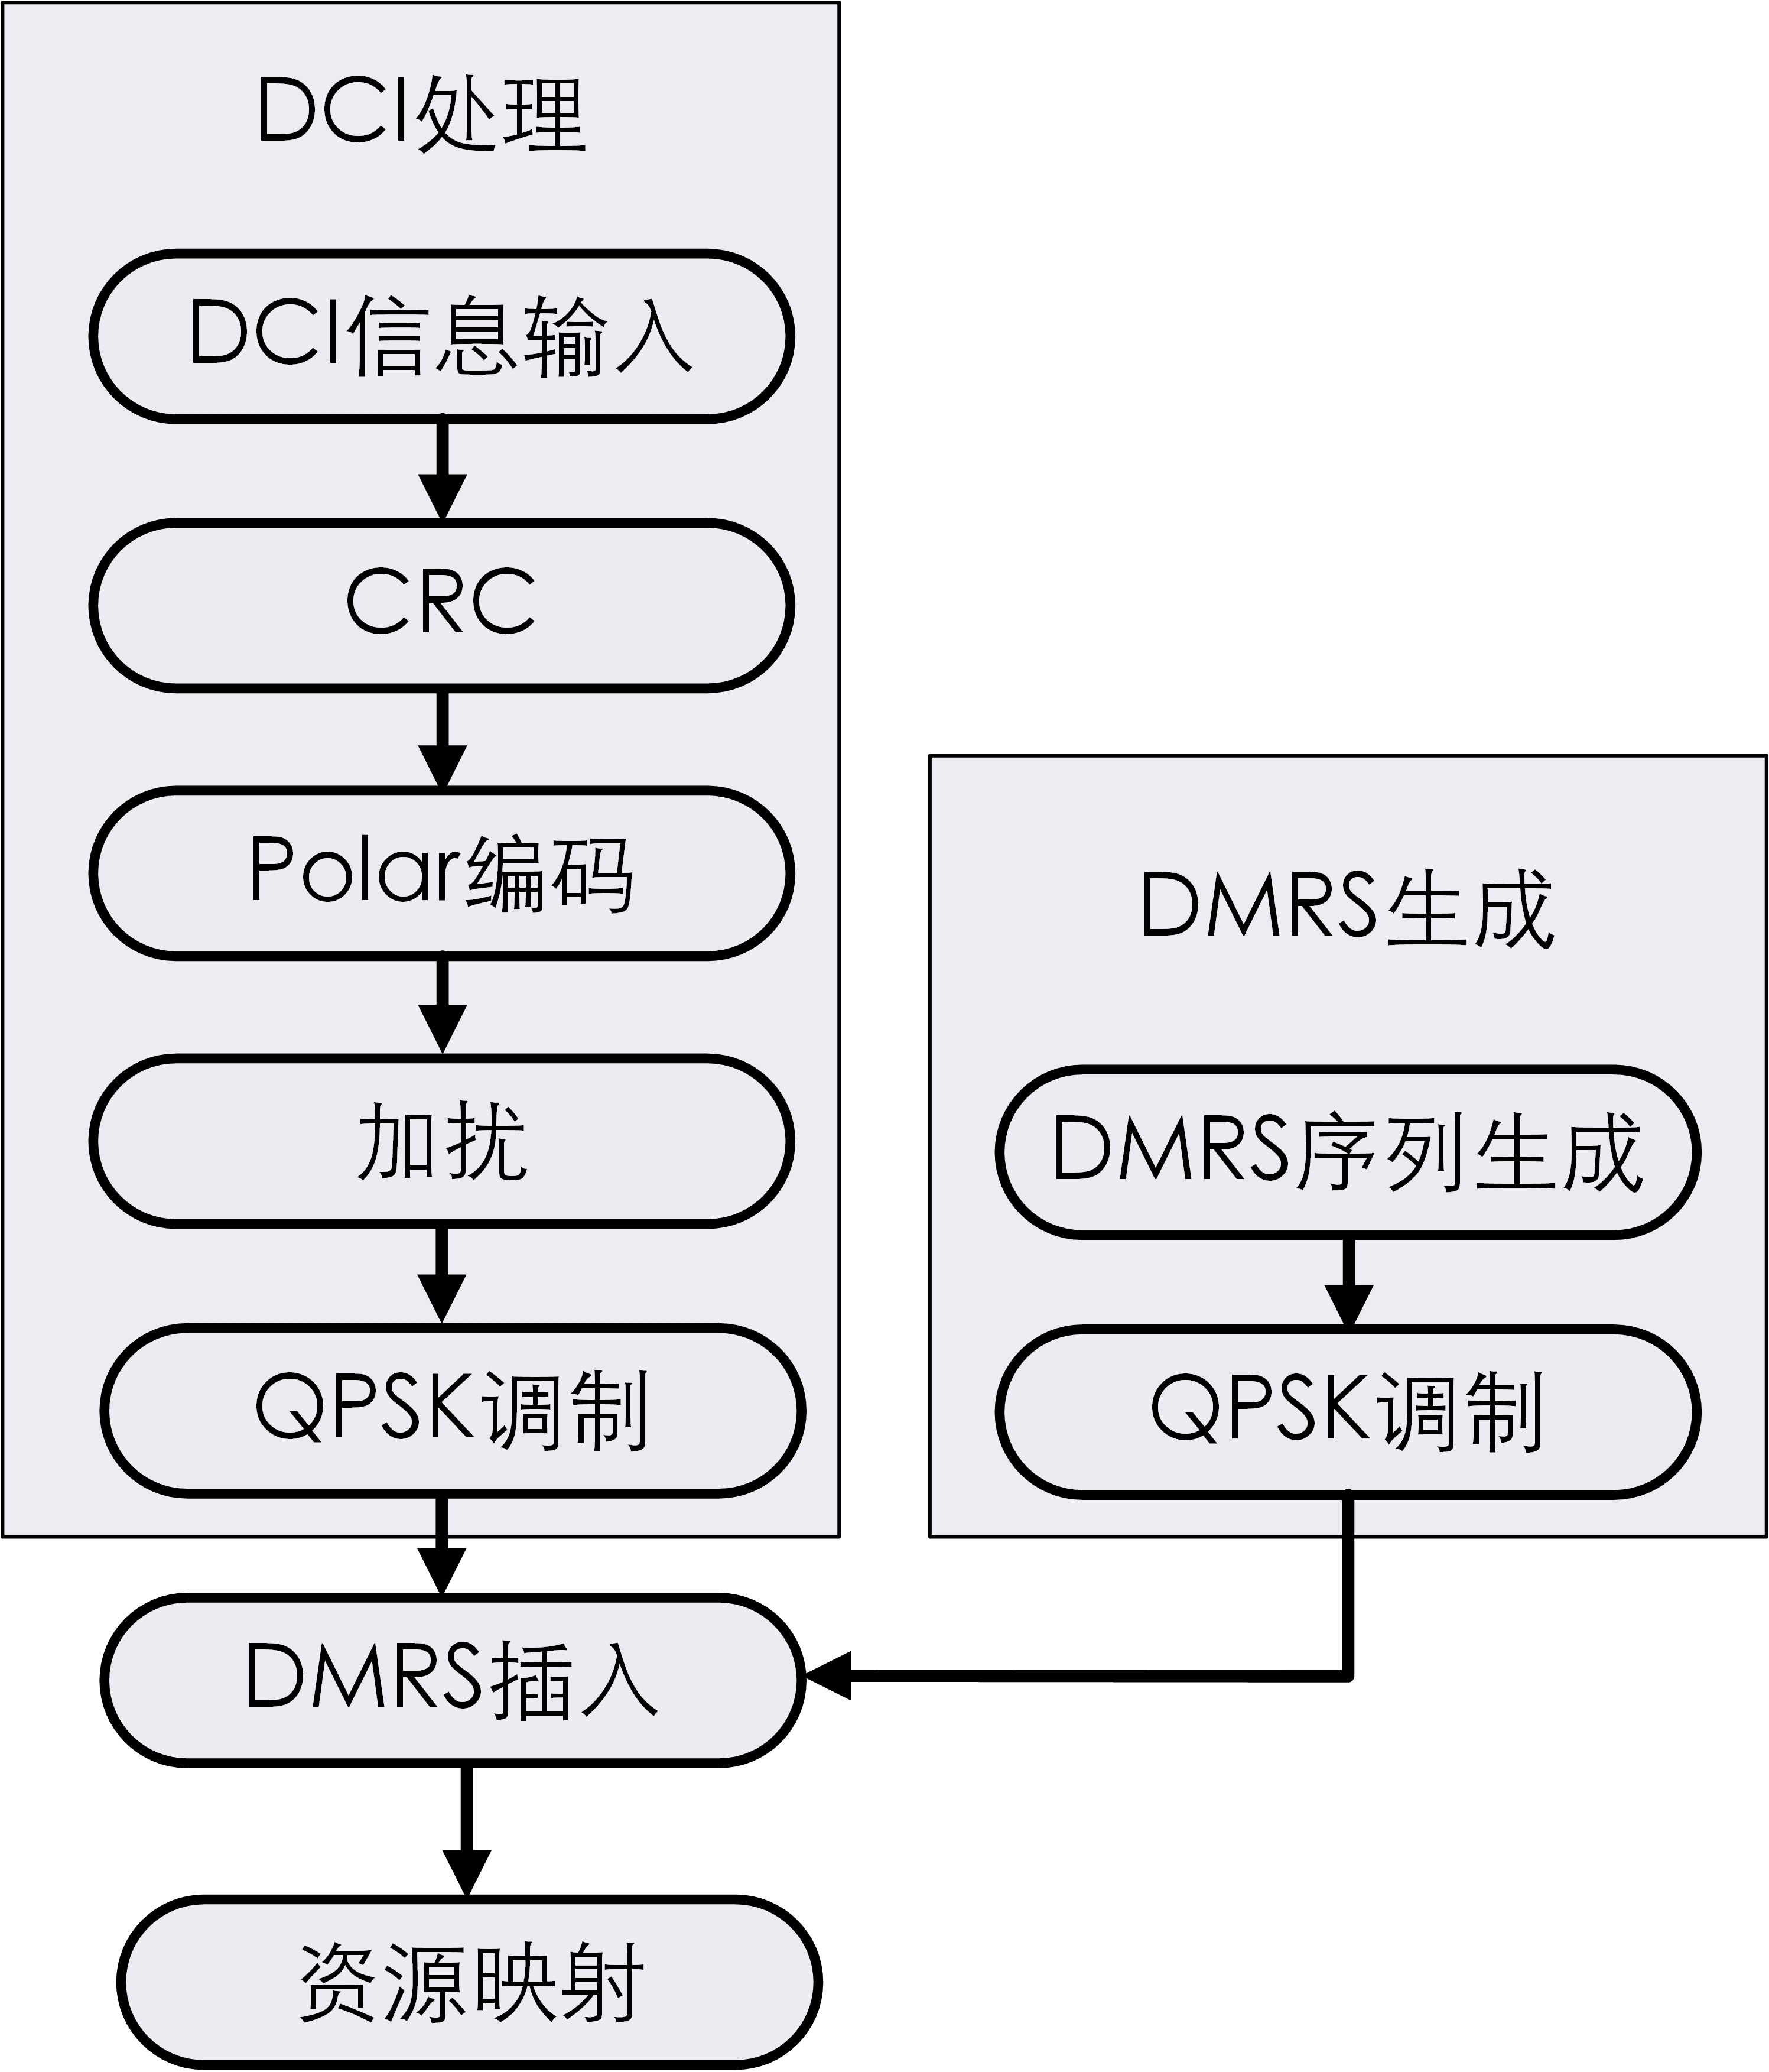
\includegraphics[width=0.5\textwidth]{nr_pdcch_process.jpg}
  \caption{图迅科技5G物理层PDCCH处理流程图}
  \label{F.1_4}
\end{figure}

\begin{table}[h]
  \centering
  \caption{PDCCH主要功能列表}
  \label{T.1_3}
  \begin{tabular}{llllll}
      \hline
        & 功能   & 支持情况 \\
      \hline
        & L2参数解析 & 支持 \\
      \hline
        & CCE-REG映射类型 & 交织,非交织 \\
      \hline
        & DCI Format & \makecell[l]{Format0\_0,  Format0\_1, Format1\_0, Format1\_1, \\ Format2\_0, Format2\_1, Format2\_2, Format2\_3}\\
      \hline
        & 聚合度 & 1,2,4,8,16 \\
      \hline
        & 预编码粒度 &  sameAsREG-bundle,allContiguousRBs \\
      \hline
        & DMRS参考点 &  CRB0,CORESET \\
      \hline
        & DMRS生成 &  序列生成,资源映射 \\
      \hline
        & PDCCH生成 &  添加CRC,polar编码,速率匹配,加扰,QPSK调制, 资源映射\\
      \hline{}
  \end{tabular}
\end{table}

C. PDSCH功能
\par
\hangafter=0 %第一行缩进
\setlength{\hangindent}{2em}
如图\ref{F.1_5}所示,PDSCH处理用户级数据信道,PDSCH DMRS和PDSCH数据一起发送,用于该数据的解调,下行PDSCH及其DMRS功能见表\ref{T.1_4}。

\begin{figure}[H]
  \centering
  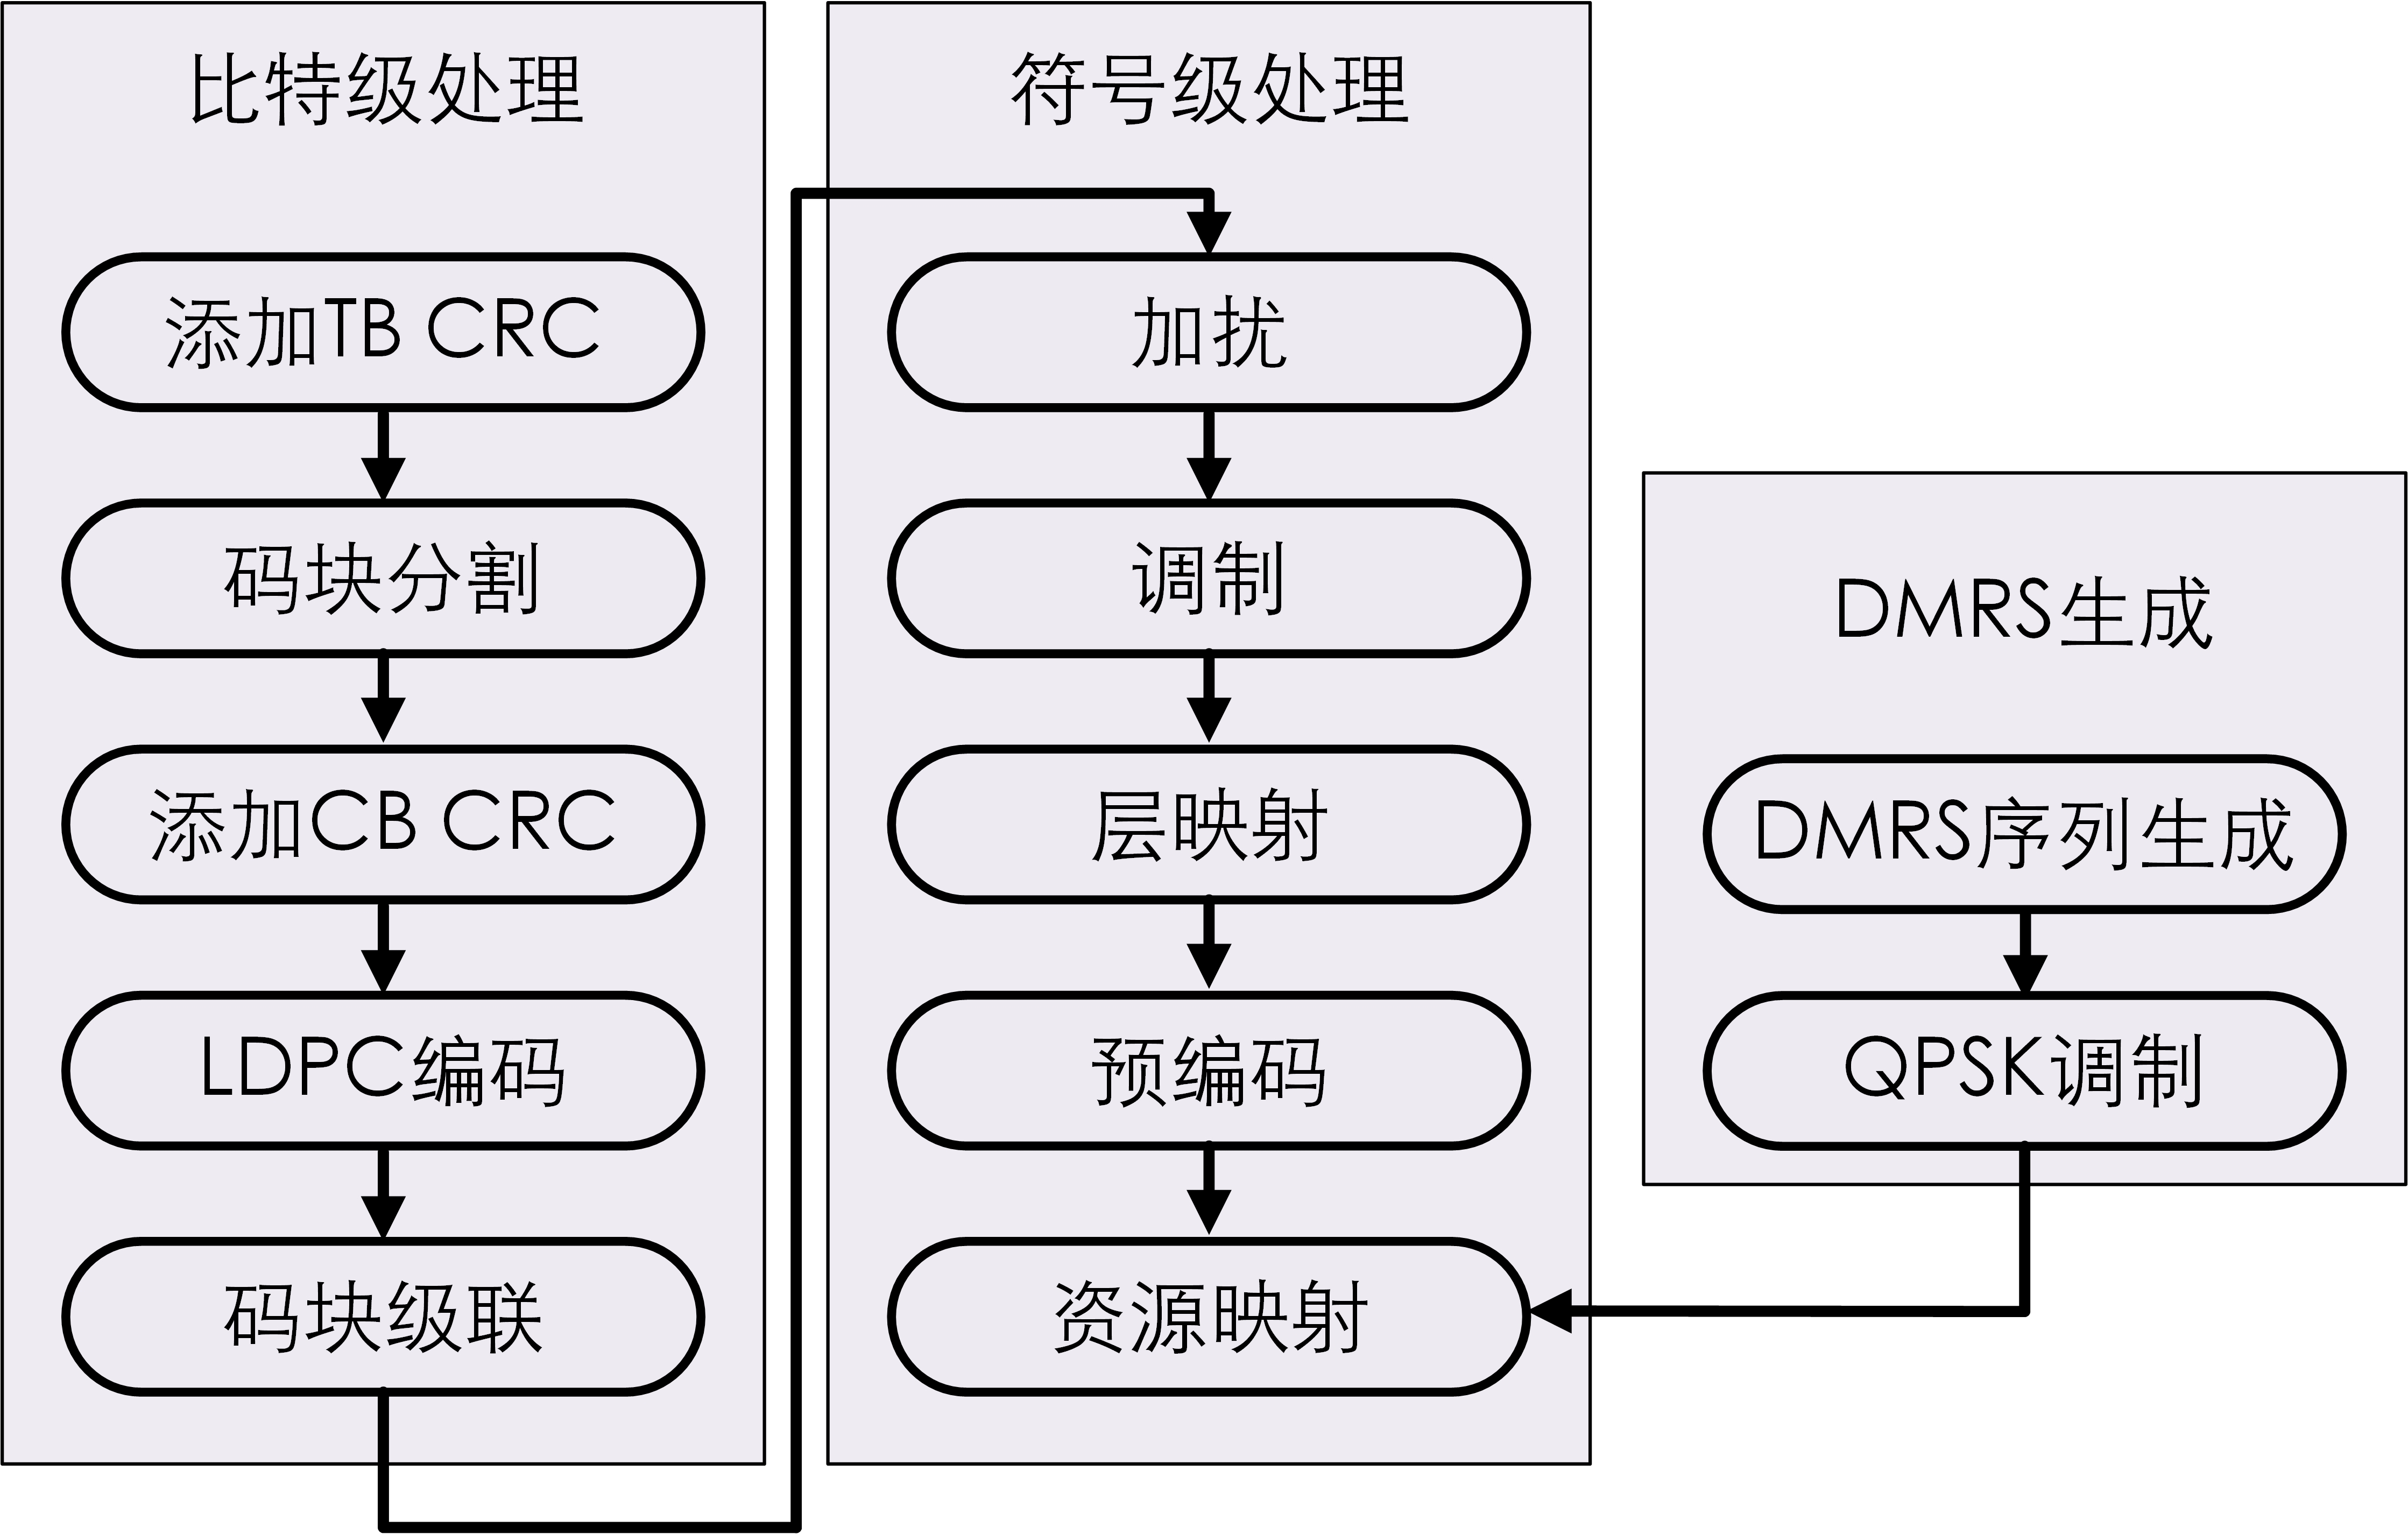
\includegraphics[width=0.7\textwidth]{nr_pdsch_process.jpg}
  \caption{图迅科技5G物理层PDSCH处理流程图}
  \label{F.1_5}
\end{figure}

\begin{table}[h]
    \centering
    \caption{PDSCH功能列表}
    \label{T.1_4}
    \begin{tabular}{llllll}
        \hline
          & 功能   & 支持情况 \\
        \hline
          & L2参数解析 & 支持 \\
        \hline
          & 添加TB CRC & CRC16,CRC24A \\
        \hline
          & 码块分割 & 码块分割,添加CRC\\
        \hline
          & LDPC编码 & basegraph1,basegraph2 \\
        \hline
          & 速率匹配 &  冗余版本0,1,2,3 \\
        \hline
          & 码块级联 &  支持 \\
        \hline
          & 加扰 &  支持 \\
        \hline
          & 调制 &  QPSK,16QAM,64QAM,256QAM \\
        \hline
          & 层映射 &  1,2,3,4层\\
        \hline
          & PDSCH频域资源分配方式 &  Type0, Type1\\
        \hline
          & PDSCH时域资源分配方式 &  Mapping TypeA, Mapping TypeB\\
        \hline
          & VRB-PRB映射 &  非交织映射\\
        \hline
          & PDSCH资源映射 &  支持\\
        \hline
          & DMRS类型 &  Type1, Type2\\
        \hline
          & 前置DMRS数量 & 1,2\\
        \hline
          & 天线端口数量 & 1,2,4\\
        \hline{}
    \end{tabular}
\end{table}

D. CSI-RS功能

\par
\hangafter=0 %第一行缩进
\setlength{\hangindent}{2em}
如图\ref{F.1_6}所示,CSI-RS处理下行信道状态参考信号,下行CSI-RS功能如表\ref{T.1_5}所示。

\begin{figure}[H]
  \centering
  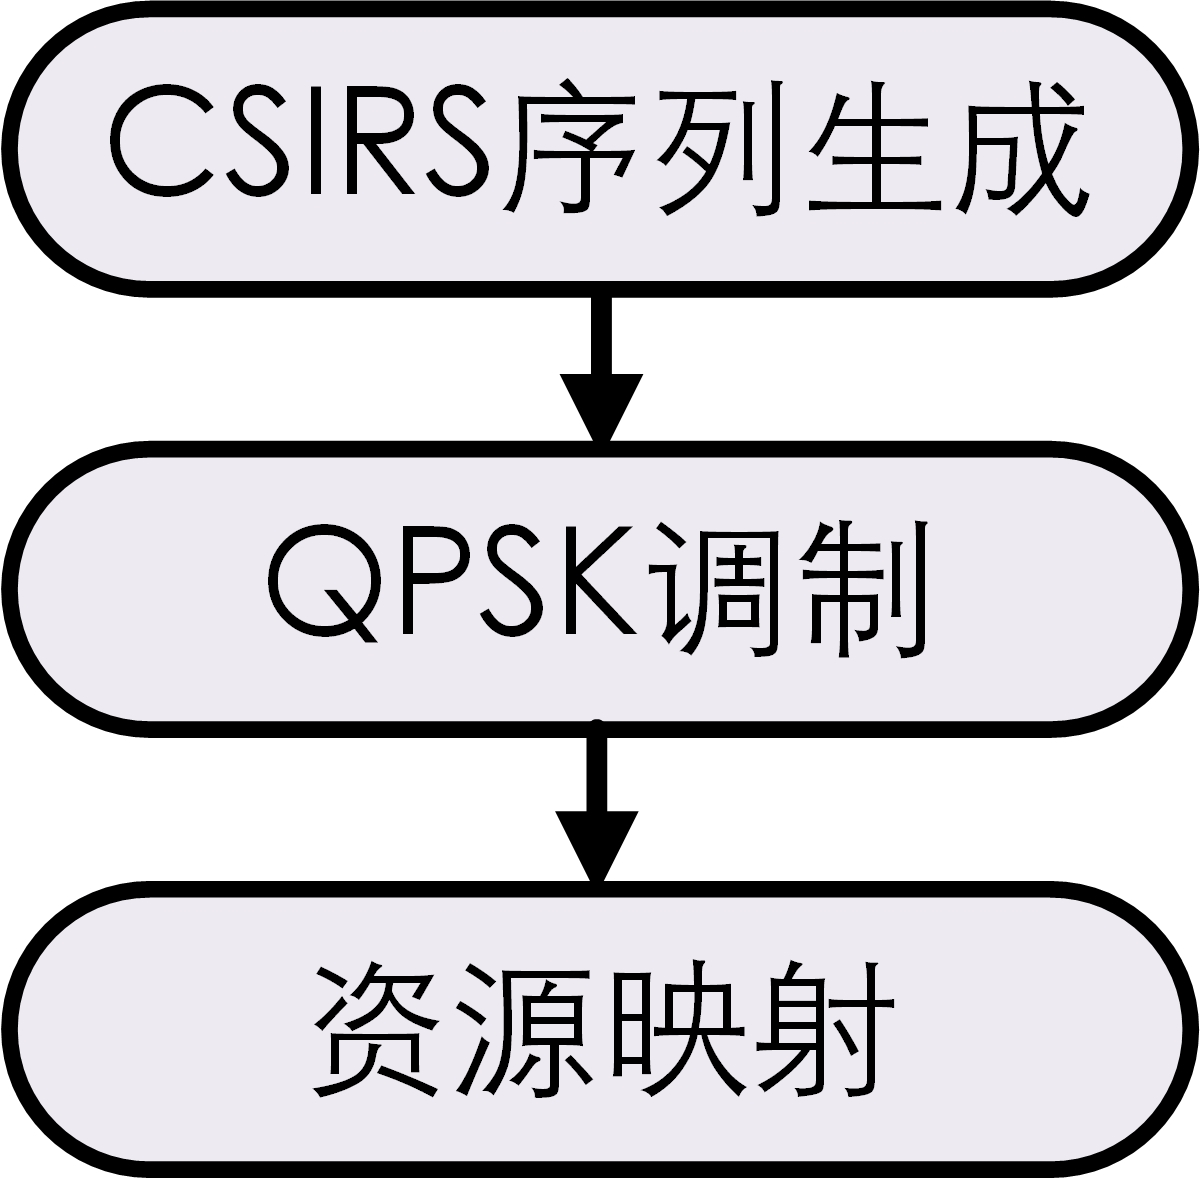
\includegraphics[width=0.2\textwidth]{nr_csirs_process.jpg}
  \caption{图迅科技5G物理层CSIRS处理流程图}
  \label{F.1_6}
\end{figure}

\begin{table}[!htbp]
    \centering
    \caption{CSI-RS功能列表}
    \label{T.1_5}
    \begin{tabular}{llllll}
        \hline
          & 功能   & 支持情况 \\
        \hline
          & L2参数解析 & 支持 \\
        \hline
          & CSI-RS端口数量 & 1,2,4,8 \\
        \hline
          & CSI-RS生成 & 序列生成,资源映射\\
        \hline{}
    \end{tabular}
\end{table}

(2) NR上行信道 

\begin{figure}[!htbp]
  \centering
  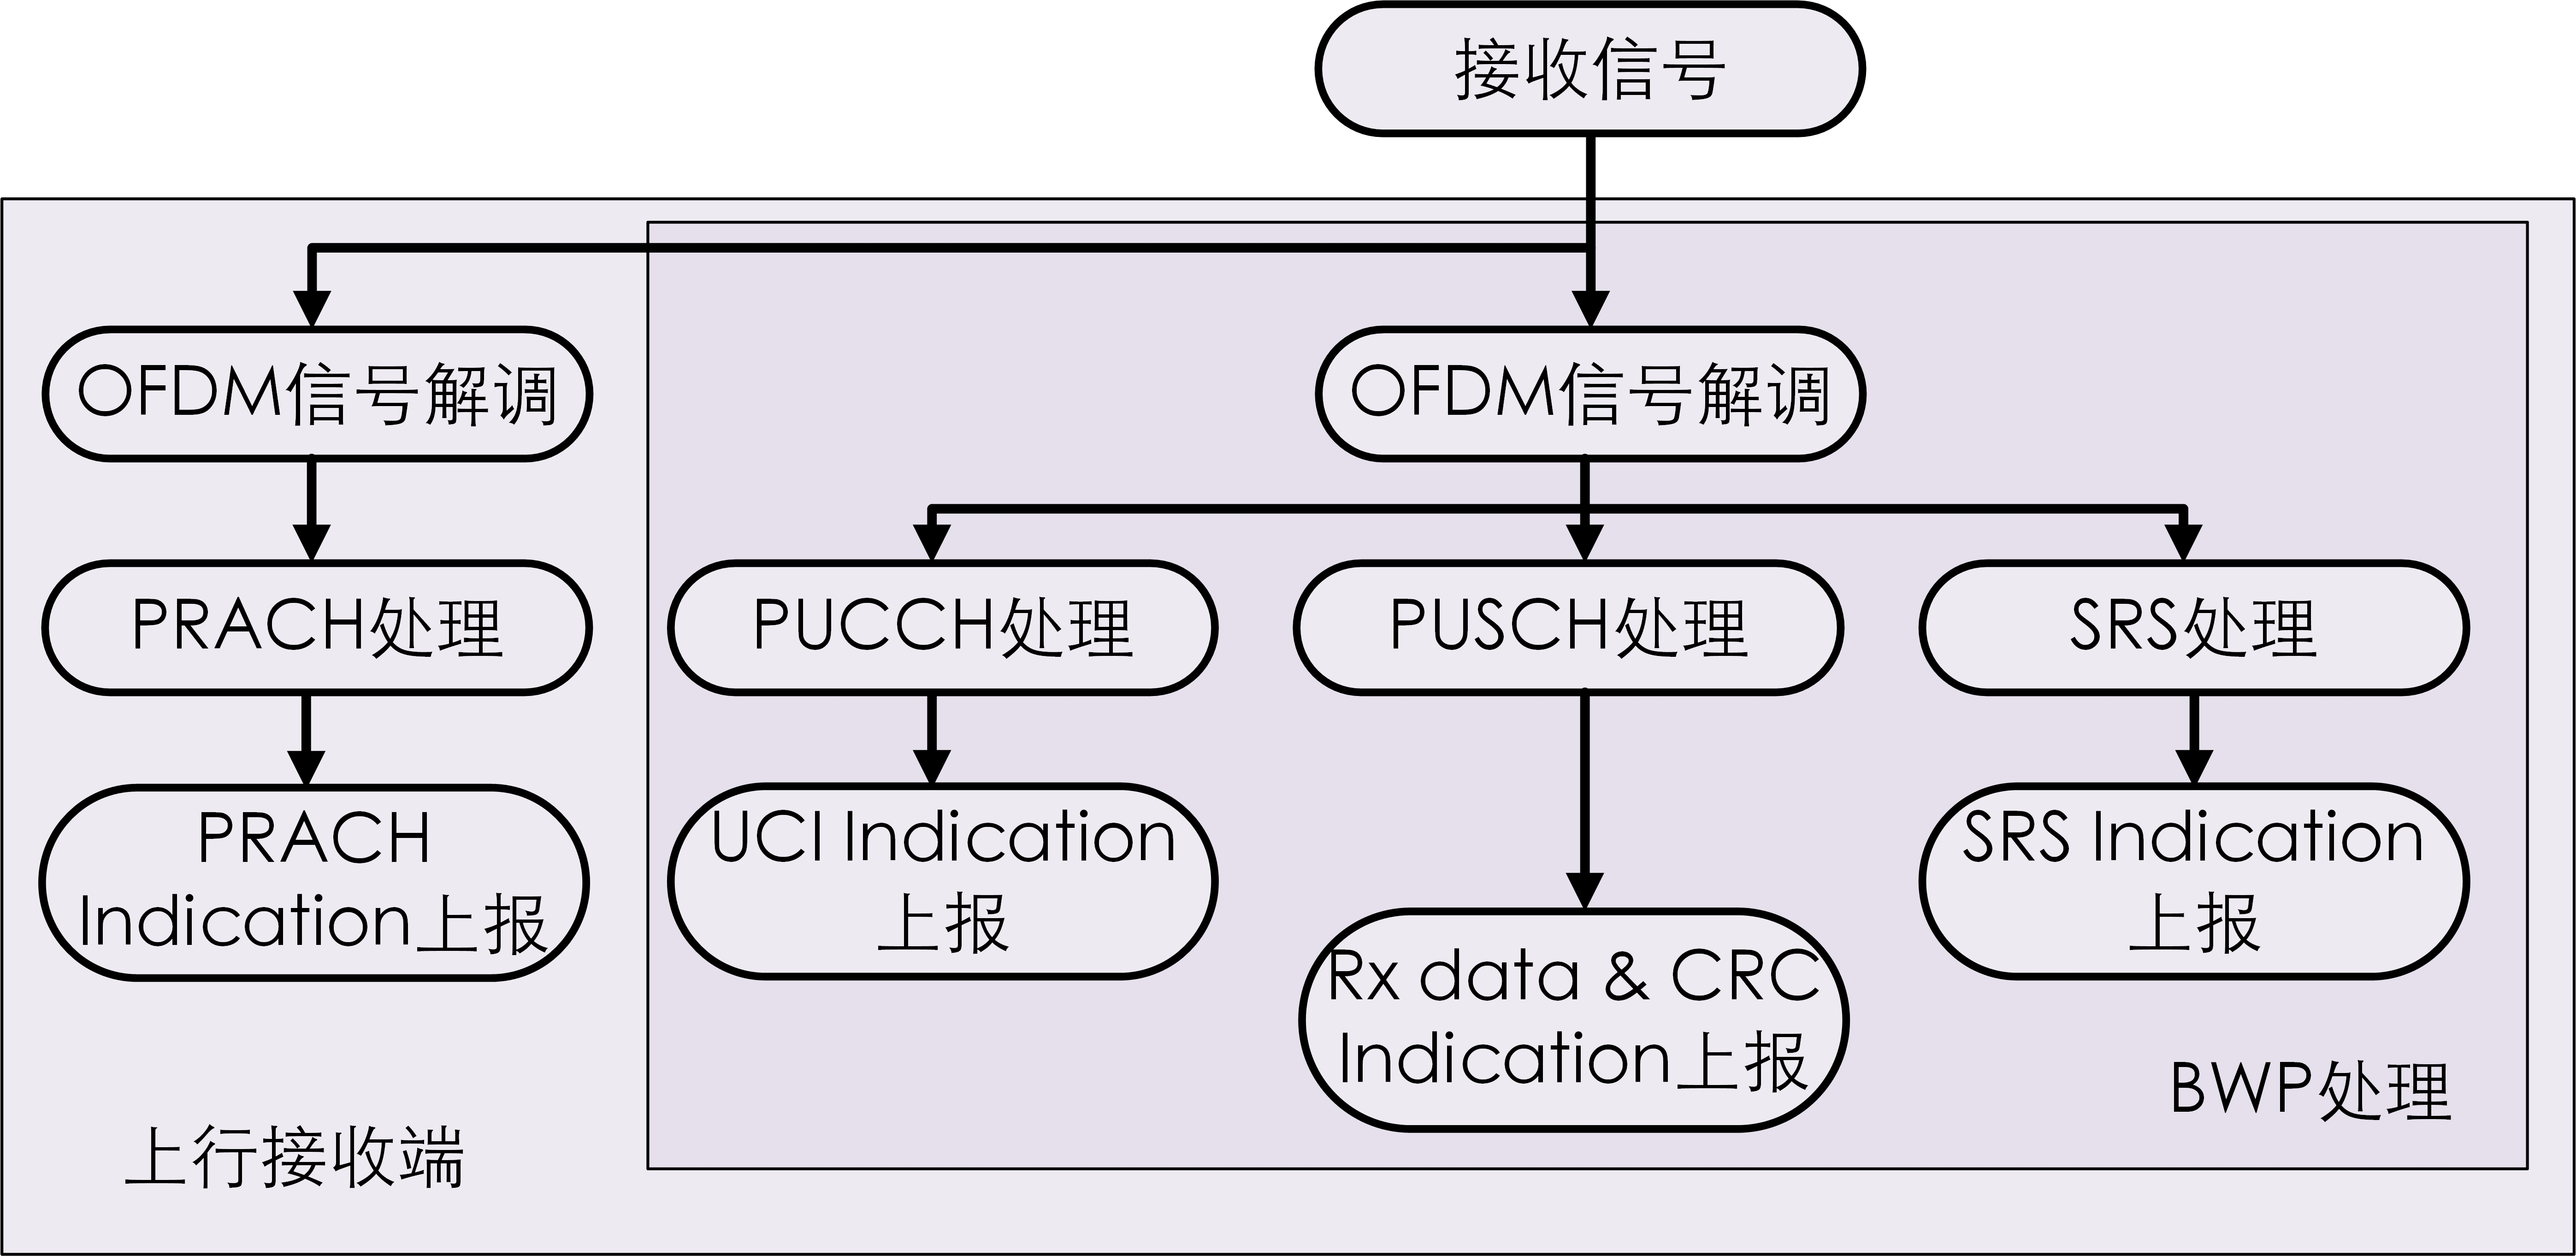
\includegraphics[width=0.8\textwidth]{nr_ul_reveiver.jpg}
  \caption{图迅科技5G物理层上行总体处理流程图}
  \label{F.1_7}
\end{figure}

\par
\hangafter=0 %第一行缩进
\setlength{\hangindent}{2em}
NR上行信道支持基于3GPP协议版本f70的基带信号解调功能(图\ref{F.1_7}),其组成部分包括:
\par
\hangafter=0 %第一行缩进
\setlength{\hangindent}{2em}
物理随机接入信道(PRACH)
\par
\hangafter=0 %第一行缩进
\setlength{\hangindent}{2em}
物理上行控制信道(PUCCH)
\par
\hangafter=0 %第一行缩进
\setlength{\hangindent}{2em}
物理上行共享信道(PUSCH)
\par
\hangafter=0 %第一行缩进
\setlength{\hangindent}{2em}
探测参考信号(SRS)

A.	PRACH功能

\par
\hangafter=0 %第一行缩进
\setlength{\hangindent}{2em}
如图\ref{F.1_8}所示,PRACH的作用是用于UE发起随机接入,其支持的功能列表如表\ref{T.1_6}所示:

\begin{figure}[H]
  \centering
  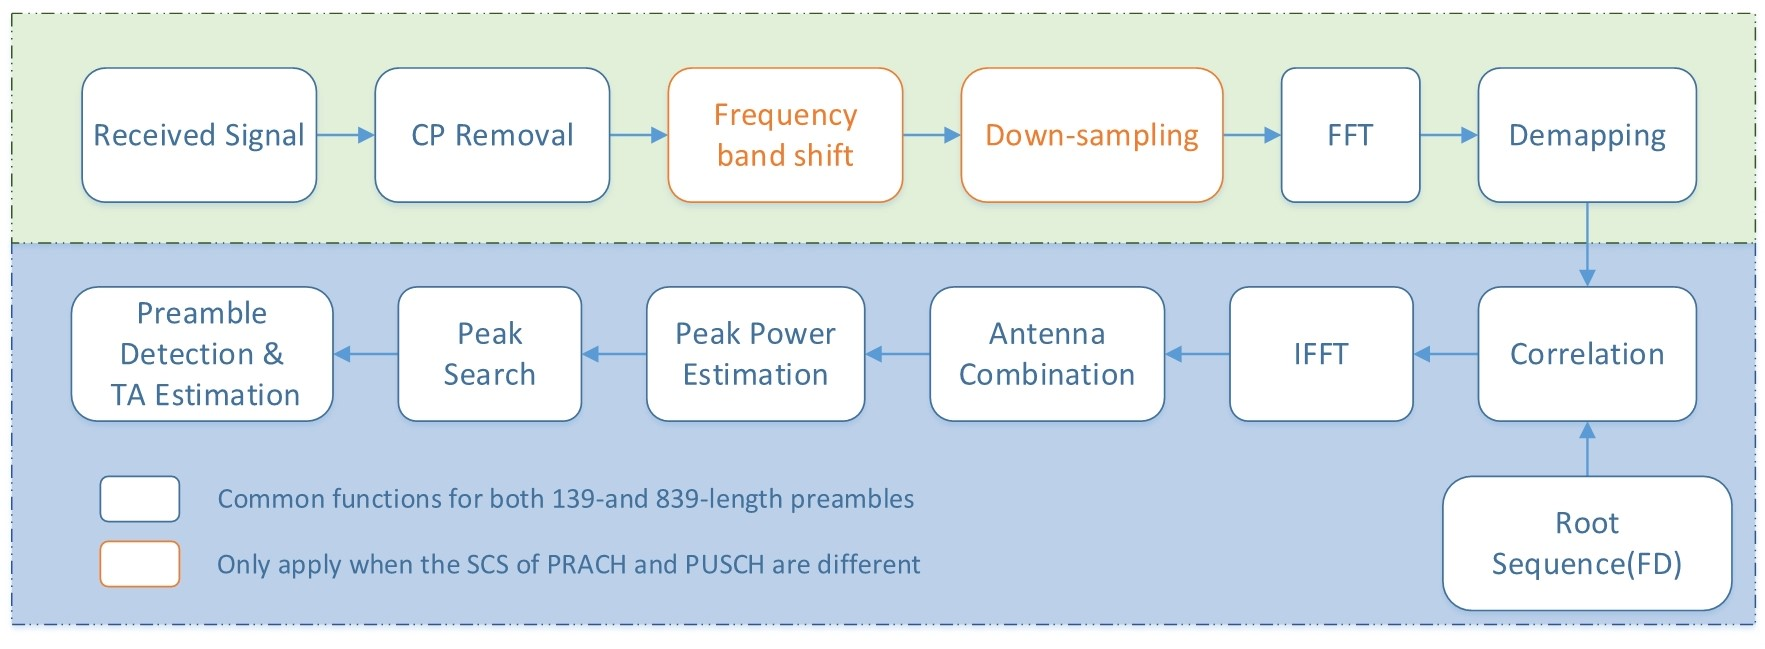
\includegraphics[width=0.8\textwidth]{nr_prach_receiver.jpg}
  \caption{图迅科技5G物理层PRACH接收处理流程图}
  \label{F.1_8}
\end{figure}

\begin{table}[htb]
    \centering
    \caption{PRACH功能列表}
    \label{T.1_6}
    \begin{tabular}{llllll}
        \hline
          & 功能   & 支持情况 \\
        \hline
          & L2参数解析 & 支持 \\
        \hline
          & PRACH格式 & 格式0/A1/A2/A3/B1/B2/B3/B4/C0/C2 \\
        \hline
          & Preamble长度 & 139(短格式),839(长格式)\\
        \hline
          & 非限制集 & 支持 \\
        \hline
          & 限制集 & Type A, Type B \\
        \hline
          & 接收机功能 & 信噪比和噪声方差估计, 峰值检测,上行定时提前量估计,频率偏移估计 \\
        \hline{}
    \end{tabular}
\end{table}

B.	PUCCH功能

\par
\hangafter=0 %第一行缩进
\setlength{\hangindent}{2em}
上行PUCCH信道只要用于传输上行控制信息(UCI),包括HARQ/SR/CSI等。图\ref{F.1_9}是PUCCH Format0的接收处理流程,图\ref{F.1_10}是PUCCH Format1的接收处理流程,图\ref{F.1_11}是PUCCH Format2/3/4的接收处理流程,上行PUCCH信道支持的功能如表\ref{T.1_7}所示。

\begin{figure}[H]
  \centering
  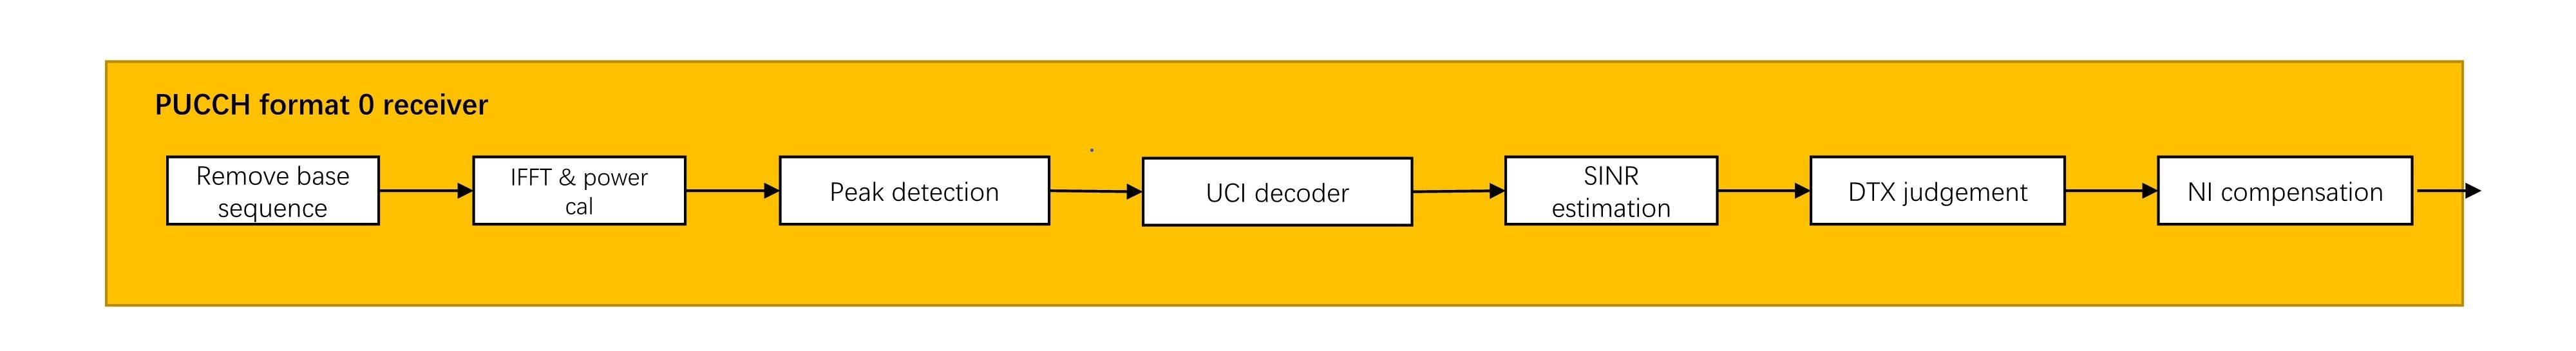
\includegraphics[width=1.0\textwidth]{nr_pucch_fmt0_receiver.jpg}
  \caption{图迅科技5G物理层PUCCH Format0接收处理流程图}
  \label{F.1_9}
\end{figure}

\begin{figure}[H]
  \centering
  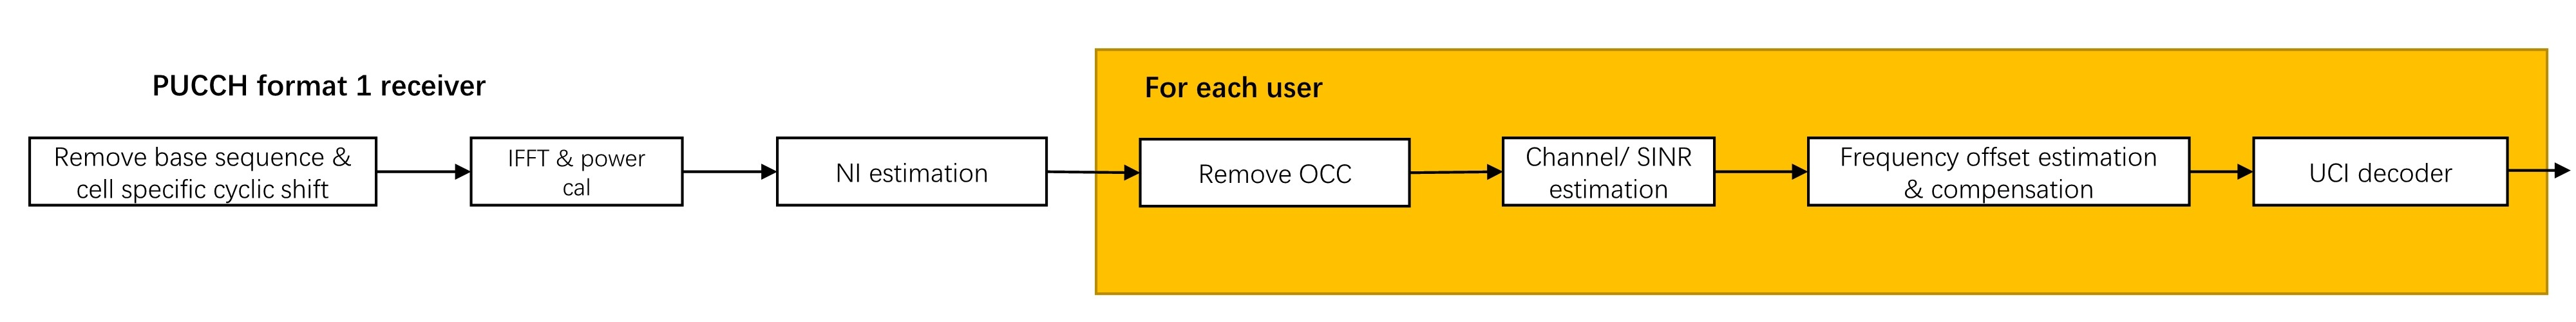
\includegraphics[width=1.0\textwidth]{nr_pucch_fmt1_receiver.jpg}
  \caption{图迅科技5G物理层PUCCH Format1接收处理流程图}
  \label{F.1_10}
\end{figure}

\begin{figure}[H]
  \centering
  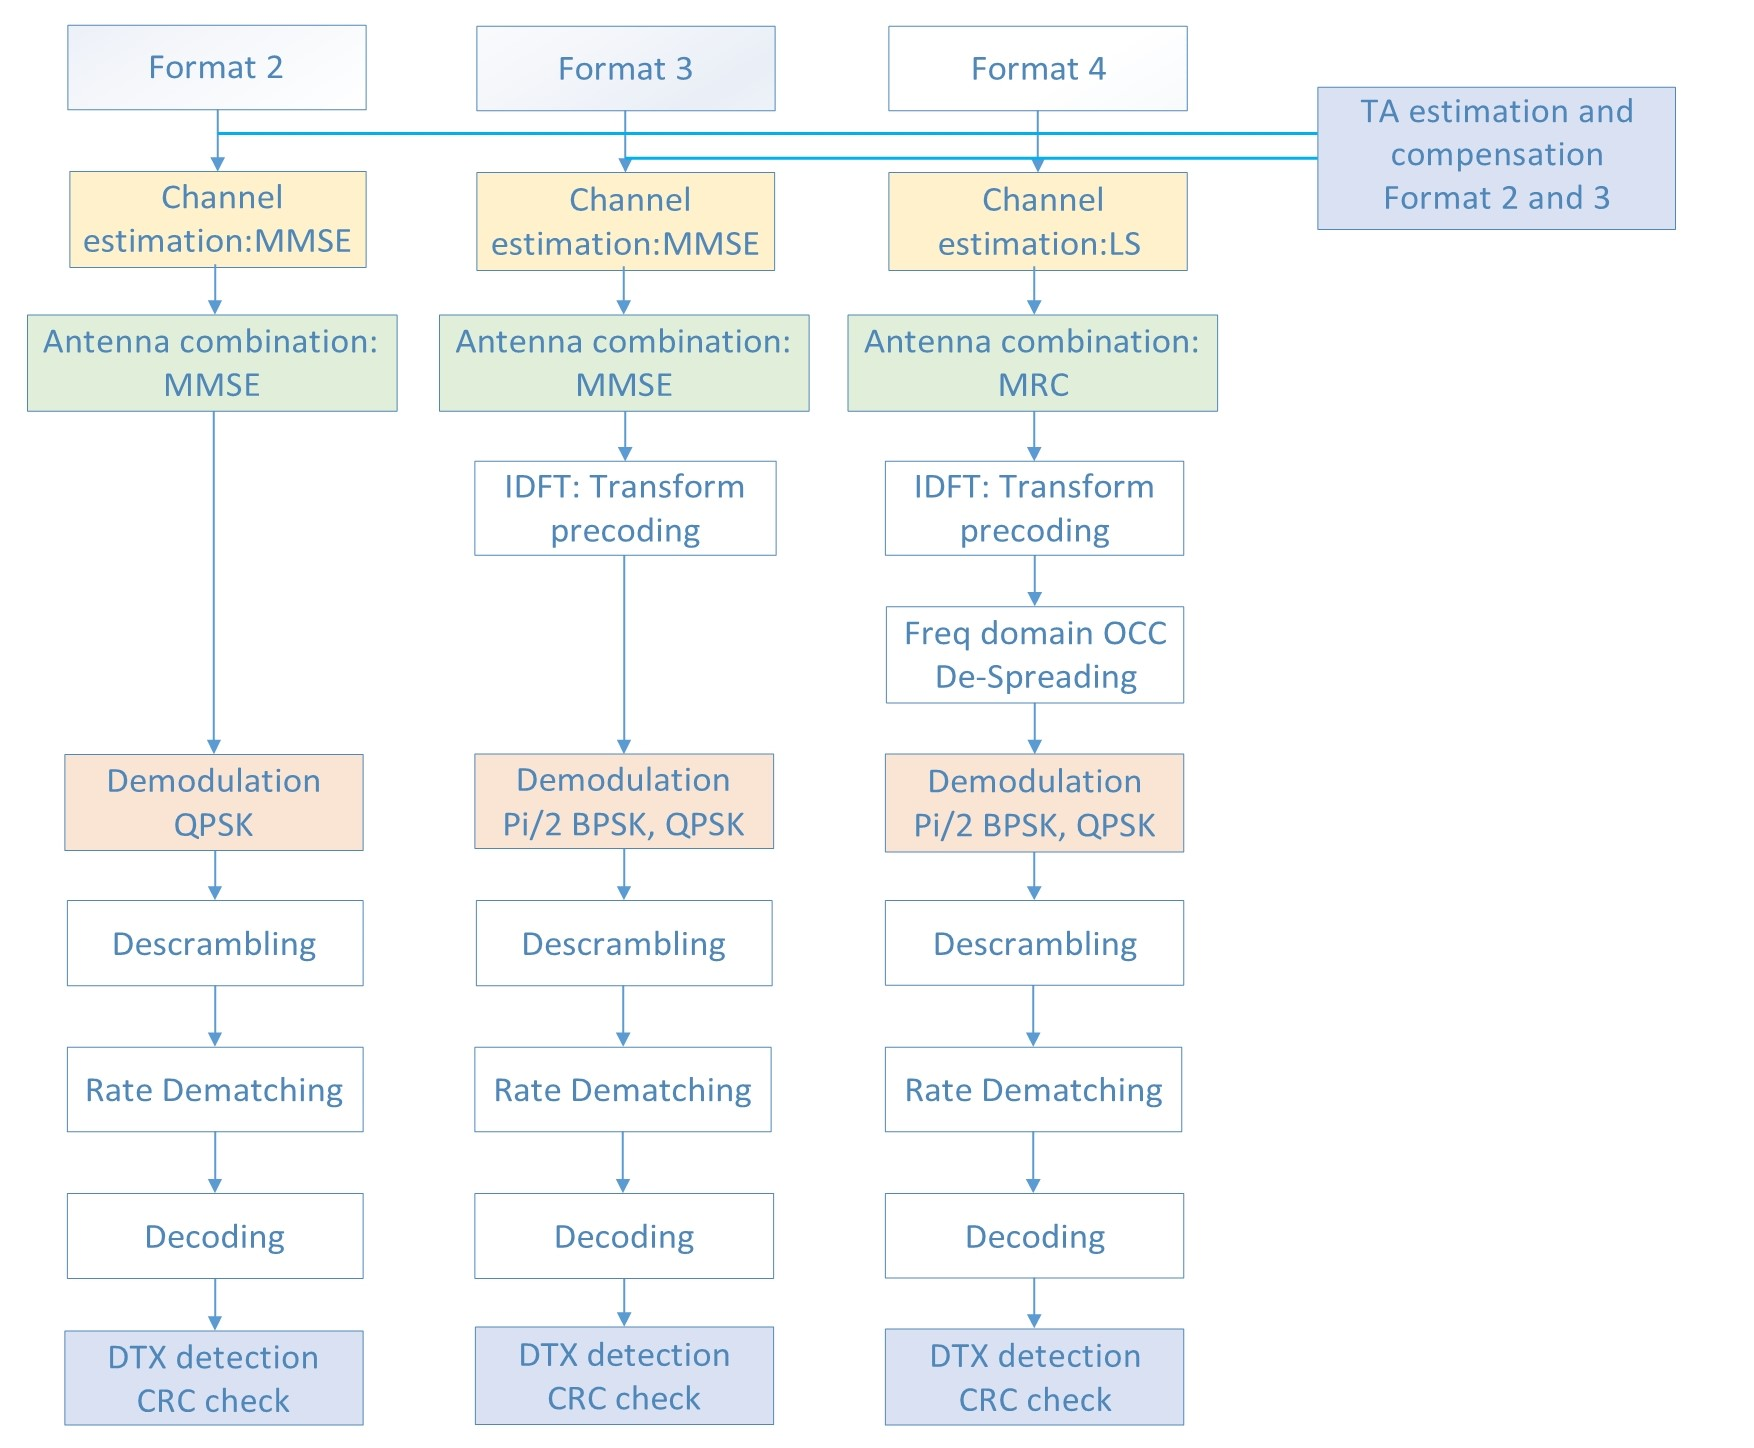
\includegraphics[width=1.0\textwidth]{nr_pucch_fmt234_receiver.jpg}
  \caption{图迅科技5G物理层PUCCH Format2/3/4接收处理流程图}
  \label{F.1_11}
\end{figure}

\begin{table}[H]
    \centering
    \caption{PUCCH功能列表}
    \label{T.1_7}
    \begin{tabular}{llllll}
        \hline
          & 功能   & 支持情况 \\
        \hline
          & L2参数解析 & 支持 \\
        \hline
          & 频率范围 & FR1 \\
        \hline
          & 子载波间隔 & 30kHz\\
        \hline
          & 带宽 & 支持100MHz, 80MHz, 60MHz, 50MHz, 40MHz, 30MHz, 20MHz灵活配置 \\
        \hline
          & PUCCH格式 & 格式0/1/2/3 \\
        \hline
          & UCI比特数 & \makecell[l]{格式0:比特数$\leq$2,\\格式1:比特数$\leq$2, \\格式2:比特数$\textgreater$2, \\格式3:比特数$\textgreater$2} \\
        \hline
          & 组跳和序列跳 & 支持 \\
        \hline
          & 信道估计 & 支持 \\
        \hline
          & 信噪比和噪声方差估计 & 支持 \\ 
        \hline
          & UCI译码 & 支持(Polar译码和SmallBlock译码) \\
          \hline{}
    \end{tabular}
\end{table}

C.	PUSCH功能支持列表

\par
\hangafter=0 %第一行缩进
\setlength{\hangindent}{2em}
如图\ref{F.1_12}所示,上行PUSCH信道主要进行上行业务数据传输,其支持的功能如表\ref{T.1_8}所示:

\begin{figure}[H]]
  \centering
  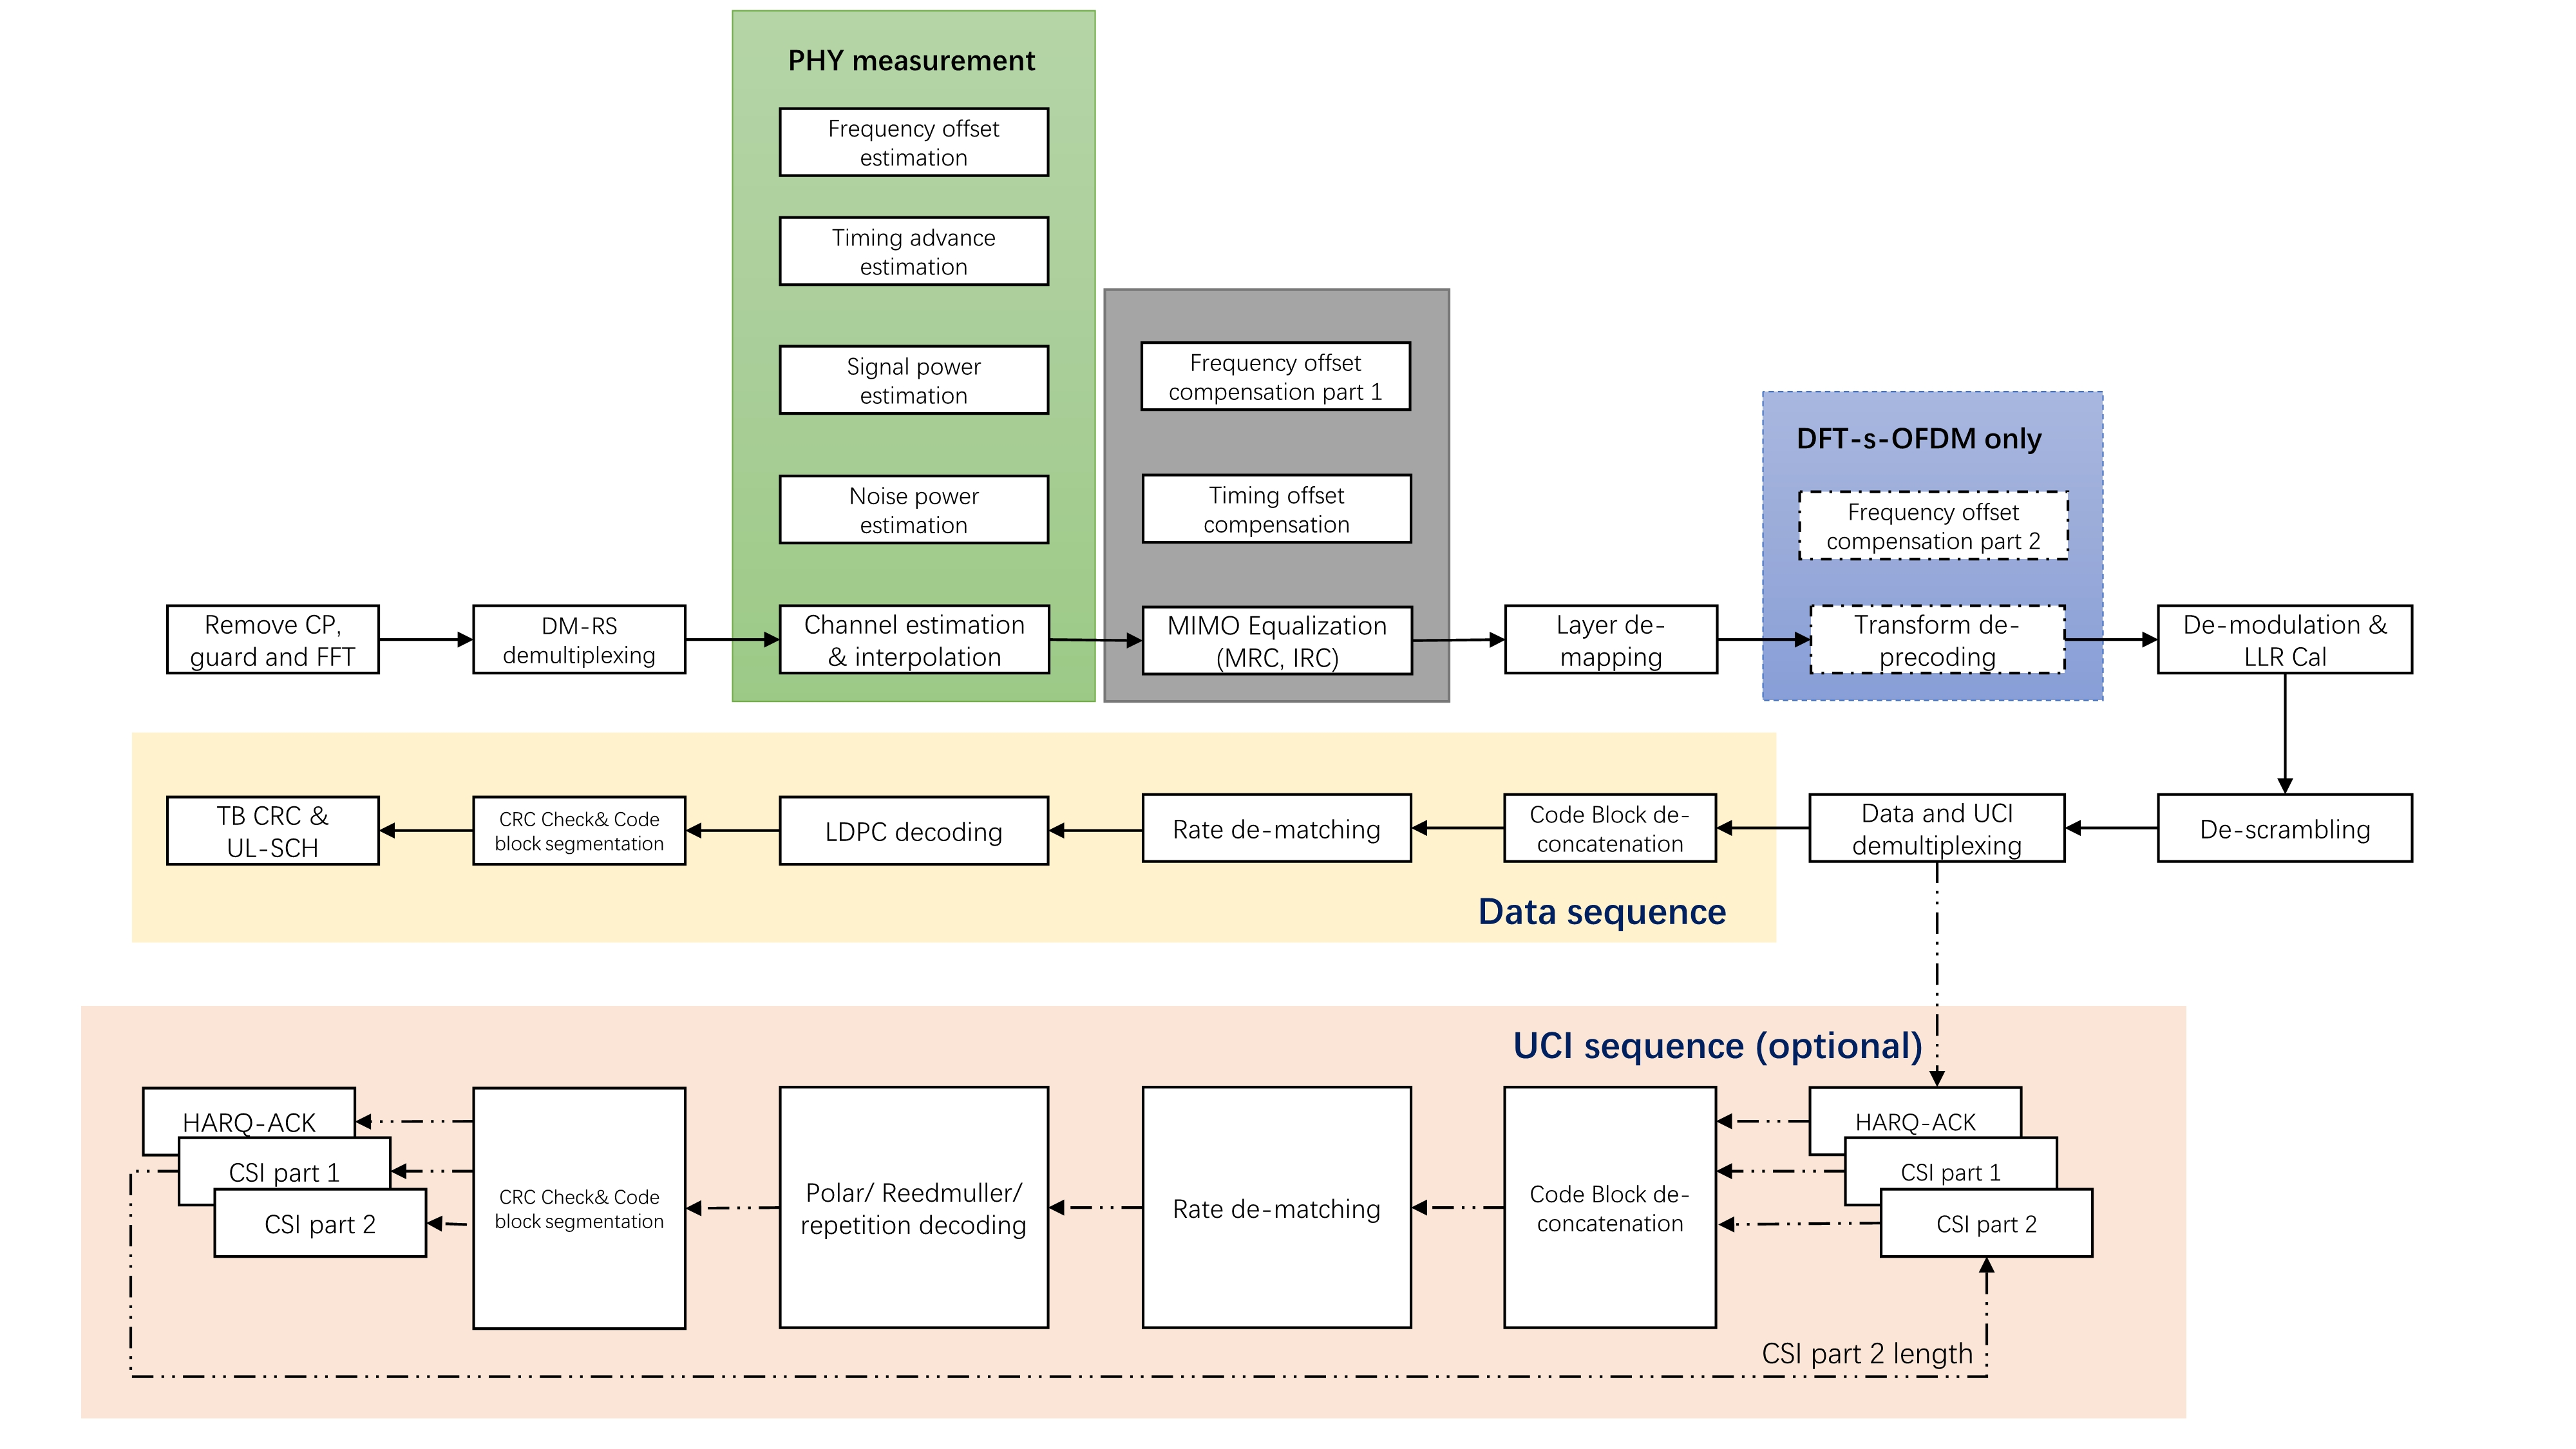
\includegraphics[width=1.0\textwidth]{nr_pusch_receiver.jpg}
  \caption{图迅科技5G物理层PUSCH接收处理流程图}
  \label{F.1_12}
\end{figure}


\begin{table}[H]
    \centering
    \caption{PUSCH功能列表}
    \label{T.1_8}
    \begin{tabular}{llllll}
        \hline
          & 功能   & 支持情况 \\
        \hline
          & L2参数解析 & 支持 \\
        \hline
          & 频率范围 & FR1 \\
        \hline
          & 子载波间隔 & 30kHz\\
        \hline
          & 带宽 & 支持100MHz, 80MHz, 60MHz, 50MHz, 40MHz, 30MHz, 20MHz灵活配置 \\
        \hline
          & OFDM波形 & CP-OFDM 和DFT-s-OFDM \\
        \hline
          & 调制方式 & pi/2-BPSK, QPSK, 16QAM, 64QAM \\
        \hline
          & PUSCH 时域资源分配类型 & Type A 和Type B \\
        \hline
          & VRB到PRB 映射 & 非交织映射 \\
        \hline
          & 上行流数 & 1,2 \\ 
        \hline
          & DMRS配置类型 & Type1 \\
        \hline
          & DMRS附加导频 & 支持 \\
        \hline
          & DFT-s-OFDM DMRS & 支持组跳频和序列跳频 \\
        \hline
          & 接收机功能 & \makecell[l]{MRC/IRC均衡,信道估计,上行定时提前量估计,频率偏移估计,\\信噪比和噪声方差估计, 频率偏移和相位噪声估计, LDPC译码} \\
        \hline{}
    \end{tabular}
\end{table}

D.	SRS功能

\par
\hangafter=0 %第一行缩进
\setlength{\hangindent}{2em}
如图\ref{F.1_13}所示,SRS主要用于信道探测,获取上行信道信息。其支持的功能如表\ref{T.1_8}所示。

\begin{figure}[H]
  \centering
  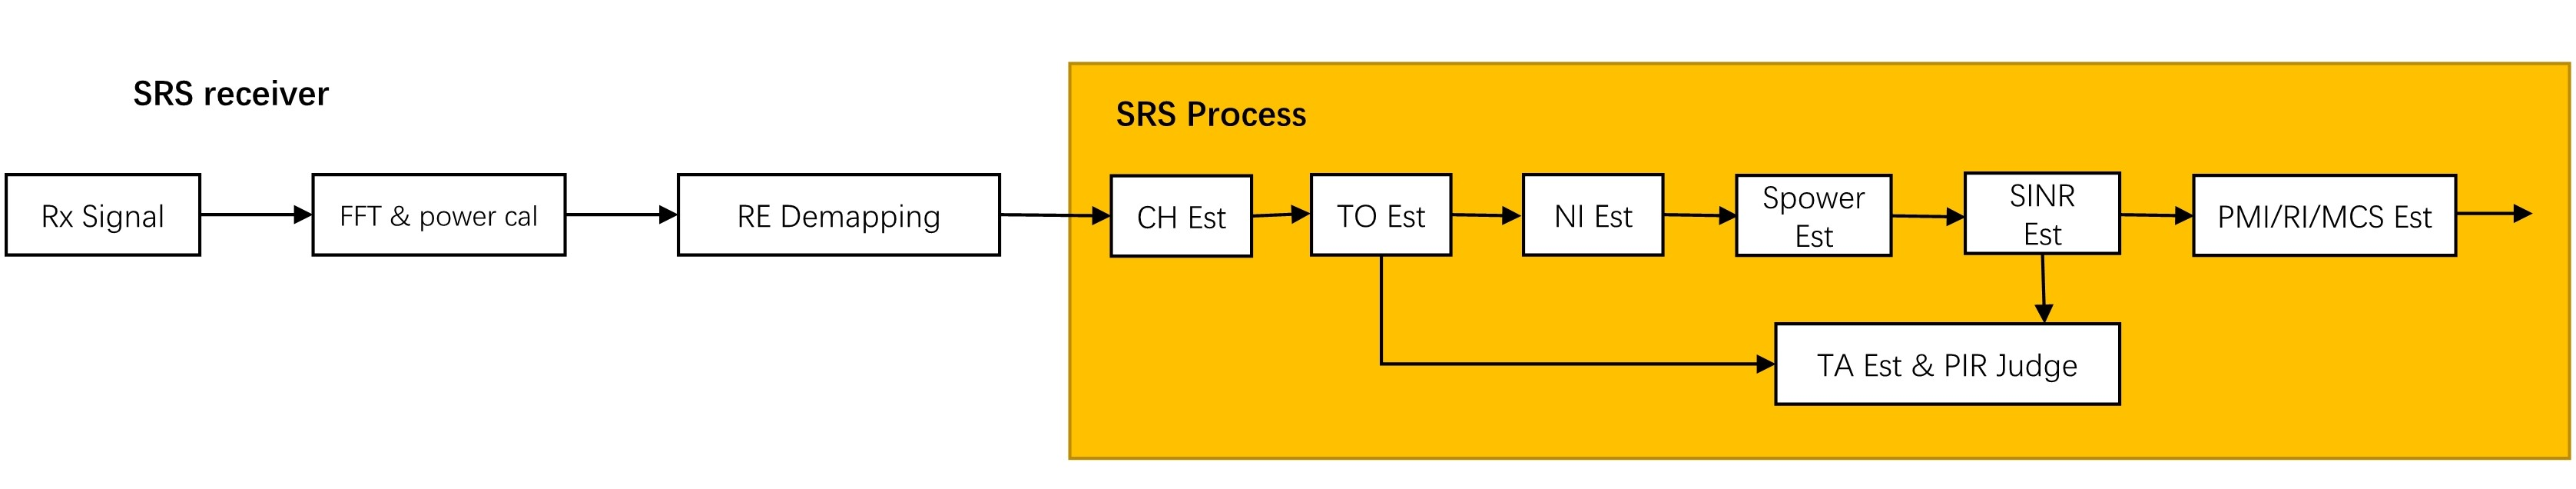
\includegraphics[width=1.0\textwidth]{nr_srs_receiver.jpg}
  \caption{图迅科技5G物理层SRS接收处理流程图}
  \label{F.1_13}
\end{figure}

\begin{table}[H]
    \centering
    \caption{SRS功能列表}
    \label{T.1_8}
    \begin{tabular}{llllll}
        \hline
          & 功能   & 支持情况 \\
        \hline
          & L2参数解析 & 支持 \\
        \hline
          & 频率范围 & FR1 \\
        \hline
          & 子载波间隔 & 30kHz\\
        \hline
          & SRS端口数 & 1/2/4 \\
        \hline
          & SRS梳状间隔 & 2/4 \\
        \hline
          & SRS符号数 & 1 \\
        \hline
          & SRS资源映射配置(C\_srs) & 0-63 \\
        \hline
          & SRS接收机功能 & 信道估计,上行定时提前量估计,信噪比和噪声方差估计 \\
        \hline{}
    \end{tabular}
\end{table}

\newpage
\section{5G物理层技术指标}
\subsection{算法性能指标}
\subsubsection{上下行协议一致性}
物理层软件的上下行协议一致性测试,要求对3GPP要求的每个信道(SSB/PDCCH/PDSCH/CSIRS/PRACH/PUCCH/PUSCH/SRS)的基带信号进行测试,满足协议规定的功能,提供功能测试列表,相应的配置参数配置文件和基带IQ数据,第三方测试软件包括但不限于MathWorks的MATLAB Toolbox,Keysight的Signal Studio/VSA等。

\subsubsection{上行接收算法性能}
链路级仿真平台的上行性能要求满足3GPP TS38.104的性能要求(以上行100MHz带宽为例):\\

% \par
% \hangafter=0 %第一行缩进
% \setlength{\hangindent}{2em}
\textbf{(1)PRACH:}
\par
\hangafter=0 %第一行缩进
\setlength{\hangindent}{2em}
PRACH仿真性能满足3GPP TS 38.104 V15.7.0中8.4节性能要求。其中虚检概率满足8.4.1节要求,检测概率满足8.4.2节中表8.4.2.2-1、表8.4.2.2-2和表8.4.2.2-3中的性能要求。
\\\textbf{(2)PUCCH}
\par
\hangafter=0 %第一行缩进
\setlength{\hangindent}{2em}
PUCCH Format 0/1/2/3仿真性能满足3GPP TS 38.104 V15.7.0中8.3节性能要求。其中DTX检测为ACK的概率满足8.3.1节要求;Format0的ACK漏检概率满足表8.3.2.2-2中要求;Format1 满足表8.3.3.1.2-2和表8.3.3.2.2-2中要求;Format2满足表8.3.4.1.2-2和表8.3.4.2.2-2中要求,Format3满足表8.3.5.2-2中要求。
\\\textbf{(3)PUSCH}
\par
\hangafter=0 %第一行缩进
\setlength{\hangindent}{2em}
PUSCH仿真性能满足3GPP TS 38.104 V15.7.0中8.2节性能要求。其中,CP-OFDM的解调性能满足8.2.1节中表8.2.1.2-7和表8.2.1.2-14中性能要求(包括1发射天线和2发射天线);DFT-s-OFDM的解调性能满足8.2.2节中表8.2.2.2-2和表8.2.2.2-4中性能要求。


\subsection{系统性能指标}

\subsubsection{下行}
100MHz带宽典型帧结构(DDDDDDDSUU)下,下行4流传输时,单用户峰值速率大于等于1.64Gbps。
\subsubsection{上行}
100MHz带宽典型帧结构(DDDDDDDSUU)下,上行2流传输时,单用户峰值速率大于等于200Mbps。

\newpage

\section{里程碑与交付件}

\subsection{5G物理层源代码}
交付的5G物理层源代码包含完整的,基于x86平台的物理层各信道处理C/C++源代码、线程池管理代码以及内存池管理等部分的源代码。
\subsection{测试工具}
测试工具交付包含完整的测试流程介绍,测试环境搭建和源代码。
\subsection{测试向量}
测试向量包含利用第3方测试工具生成的测试参考向量,以及测试对比源码。
\subsection{Debug工具}
Debug工具包含完整的OAM工具、PHY Log抓取和分析工具的使用说明的源代码。
\subsection{交付文档}

\begin{table}[htb]
    \centering
    \caption{交付文档列表}
    \label{T.3_1}
    \begin{tabular}{llllll}
        \hline
          & 文档编号  & 文档名称   & 描述    \\
        \hline
        1 & TSNR-SYM-001 & 系统设计文档 & 5G物理层系统架构设计描述 \\
        \hline
        2 & TSNR-SYM-002 & 系统集成说明文档 & \makecell[l]{系统集成文档主要描述了物理层与上层协议栈\\的接口消息定义,与协议栈的交互流程等说明。 }\\
        \hline
        3 & TSNR-SYM-003 & 环境搭建说明文档 & \makecell[l]{环境搭建说明文档主要介绍操作系统配置,\\编译环境以及第三方软件的配置方法,配置脚本\\文件的使用说明等。}\\
        \hline
        4 & TSNR-ALG-001 & 算法方案设计说明书 & 描述物理层上行信道的基带信号处理算法和流程 \\
        \hline
        5 & TSNR-ALG-002 & 算法性能仿真测试报告 & \makecell[l]{物理层软件运行3GPP无线性能case结果报告\\物理层软件进行协议一致性测试结果报告} \\
        \hline
        6 & TSNR-TEST-001 & 测试工具说明文档 & \makecell[l]{介绍物理层软件的各级测试流程以及操作步骤} \\
        \hline
        7 & TSNR-TEST-002 & 测试向量生成说明文档 & \makecell[l]{描述协议一致性测试以及无线性能测试的参考向量\\说明和生成方式介绍} \\
        \hline{}
    \end{tabular}
\end{table}

\subsection{里程碑}
里程碑是指交易达成后按阶段交付物理层软件过程中各个阶段的交付日期和交付内容。

\subsubsection{里程碑1}
\textbf{交付日期:}待定。
\newline
\setlength{\hangindent}{2em}
\textbf{交付内容:}
\newline
\setlength{\hangindent}{2em}
(1) 5G物理层二进制\\
(2)	5G物理层测试工具。\\
(3)	5G物理层debug工具。 


\subsubsection{里程碑2}
\textbf{交付日期:}待定。
\newline
\setlength{\hangindent}{2em}
\textbf{交付内容:}
\newline
\setlength{\hangindent}{2em}
(1) 使用图迅5G物理层二进制与 第三方L2L3 协议栈、模拟核心网集成完成。\\
(2) 使用图迅5G物理层二进制与 第三方EU/RRU 集成完成。\\
(3) 使用图迅5G物理层二进制实现5G 小基站打通 one call。

\subsubsection{里程碑3}
\textbf{交付日期:}待定。
\newline
\setlength{\hangindent}{2em}
\textbf{交付内容:}
\newline
\setlength{\hangindent}{2em}
(1)	5G物理层源码。\\
(2)	5G物理层测试用例。\\
(3)	5G物理层软件相关技术文档,详见表\ref{T.3_1}。\\
(4)	5G物理层测试工具源码。\\
(5)	5G物理层debug工具源码。


\subsubsection{里程碑4}
(1)	5G端到端集成测试,包括3GPP功能测试、RAN4性能测试报告。

\newpage

\section{报价与付款流程}
\subsection{报价}
5G物理层软件各项目报价清单由表\ref{T.3_2}列出。
\begin{table}[H]
  \centering
  \caption{图迅科技5G物理层软件分项报价表}
  \label{T.3_2}
  \begin{tabular}{llllll}
      \hline
        & 项目  & 价格(RMB, 万元)   \\
      \hline
      1 & 5G物理层二进制 & 30  \\
      \hline
      2 & 5G物理层源码 & 270  \\
      \hline
      3 & 测试工具套件 & 40  \\
      \hline
      4 & 测试向量 & 30 \\
      \hline
      5 & debug工具 & 30\\
      \hline
      6 & 文档 & 50\\
      \hline
      7 & 技术支持 & 50\\
      \hline
      & 总计   &   500  \\
      \hline{}
  \end{tabular}
\end{table}

注1:技术支持包括支持协议栈集成,支持EU/RRU集成,用COST UE打通one call。\\
\newline
\setlength{\hangindent}{2em}
注2:除注1中所列的项目之外,其他项目(如实验室系统测试,运营商入网测试,商用部署的技术支持等)如需技术支持,费用由双方协商。

\subsection{付款流程}
各里程碑的付款比例如下:
\newline
\setlength{\hangindent}{2em}
里程碑1:支付合同金额的2\%。
\newline
\setlength{\hangindent}{2em}
里程碑2:支付合同金额的3\%。
\newline
\setlength{\hangindent}{2em}
里程碑3:支付合同金额的65\%。
\newline
\setlength{\hangindent}{2em}
里程碑4:支付合同金额的30\%。
\newline
\setlength{\hangindent}{2em}

\newpage
\section{售后服务}
\subsection{维保期}

2年内或者首次完成运营商入网测试(或同等测试),免费提供5G物理层软件的bug修复版本。\\

\subsection{培训}
免费提供40小时的技术培训,帮助买方理解5G物理层系统设计、算法设计以及测试流程等。

\subsection{技术支持}
(1) 支持L2/L3协议栈集成
\newline
\setlength{\hangindent}{2em}
协助买方集成第三方L2/L3协议栈软件。
\newline
(2) 支持EU/RRU集成
\newline
\setlength{\hangindent}{2em}
协助买方集成第三方EU/RRU。
\newline
\setlength{\hangindent}{2em}
(3) 使用COST UE打通one call。
\newline
\setlength{\hangindent}{2em}
(4) 支持5G小基站端到端测试
\newline
\setlength{\hangindent}{2em}
协助买方进行5G小基站端到端测试,双方根据工作量确认技术支持费用。
(5) 功能扩展升级
\newline
\setlength{\hangindent}{2em}
协助买方升级5G物理层,双方根据工作量确认技术支持费用。

\newpage
}

%%%%%%%%%%%%%%%%%%%%%%%%%%%%%%%%%%%%%%%%%%%%%%%%%%
% 临时标签,用于编译时追踪正文末尾
%%%%%%%%%%%%%%%%%%%%%%%%%%%%%%%%%%%%%%%%%%%%%%%%%%

%%%%%%%%%%%%%%%%%%%%%%%%%%%%%%%%%%%%%%%%%%%%%%%%%%
% 后续内容,标题三号黑体居中,章节无编号
% --------------------------------------------%

% https://www.zhihu.com/question/29413517/answer/44358389 %
% 说明如下:
% secnumdepth 这个计数器是 LaTeX 标准文档类用来控制章节编号深度的。在 article 中,这个计数器的值默认是 3,对应的章节命令是 \subsubsection。也就是说,默认情况下,article 将会对 \subsubsection 及其之上的所有章节标题进行编号,也就是 \part, \section, \subsection, \subsubsection。LaTeX 标准文档类中,最大的标题是 \part。它在 book 和 report 类中的层级是「-1」,在 article 类中的层级是「0」。这里,我们在调用 \appendix 的时候将计数器设置为 -2,因此所有的章节命令都不会编号了。不过,一般还是会保留 \part 的编号的。所以在实际使用中,将它设置为 0 就可以了。

% 在修改过程中请注意不要破环命令的完整性

\renewcommand\appendix{\setcounter{secnumdepth}{-2}}
\appendix

% 主文件有代码去掉页眉章节编号的“.”,但这会因为bug导致无编号章节显示一个错误编号,所以这里在无编号章节之前再次重定义sectionmark。
\renewcommand{\sectionmark}[1]{\markright{#1}}

% section 标题从这里往后改为三号黑体居中
\titleformat{\section}{\centering \zihao{3}\heiti}{\thesection}{1em}{}

% \section{参考文献} % bibliography会自动显示参考文献四个字
\addcontentsline{toc}{section}{参考文献} % 由于参考文献不是section,这句把参考文献加入目录
% \nocite{*} % 该命令用于显示全部参考文献,即使文中没引用
% cls文件中已经引入package,这里不需要调用 \bibliographystyle 了。
% \bibliographystyle{gbt7714-2005} 
\bibliography{references}
% \newpage

% \include{content/additional}

\end{document}
